\section{ACER}
\label{sACER}

\hypertarget{sACERhy}{The}
ACER\index{ACER|textbf} module prepares libraries in ACE format (A Compact
ENDF)\index{ACE format} for the MCNP\index{MCNP} continuous-energy
neutron-photon Monte Carlo code\cite{MCNP}.\index{Monte Carlo}
One of the design goals for MCNP has been to use the most detailed
representation of the physics of a problem that is practical.
Therefore, the ACE format has evolved to include all the details
of the ENDF\cite{ENDF102} representations for neutron and photon data.
However, for the sake of efficiency, the representation of data in ACE
is quite different from that in ENDF.  The fundamental difference is
the use of random access with pointers to the various parts of the
data.  Other key differences include the use of union energy grids,
equal-probability bins, and cumulative probability distributions.

This chapter describes the ACER module in NJOY2016.0.

\subsection{ACER and ACE Data Classes}
\label{ssACER_classes}

The ACE format provides for several different ``classes'' of data,
the most popular being the ``continuous-energy neutron'' class.
Others include include photo-atomic data, thermal data, and
photo-nuclear data.  Files for each class of data are distinguished
by a code letter at the end of the ZAID identifier for each material.
For example, a file with a ZAID identifier of ``13027.00c'' would
contain continuous-energy neutron data.  The data classes currently
handled by ACER and the class suffixes are given in Table~\ref{classes}.

\begin{table}[b]
\caption[ACE Data Classes and ZAID suffixes]{ACE Data Classes and ZAID suffixes}
\label{classes}
\begin{center}
\begin{tabular}{cl}
Suffix & ACE Data  Class \\
\hline
  c  &  continuous-energy neutron data \\
  t  &  thermal $S(\alpha,\beta)$ data \\
  y  &  dosimetry data \\
  p  &  photo-atomic data (incomplete) \\
  u  &  photonuclear data \\
  h  &  continuous-energy proton data \\
  o  &  continuous-energy deuteron data \\
  r  &  continuous-energy triton data \\
  s  &  continuous-energy $^{3}$He data \\
  a  &  continuous-energy alpha data \\
\hline
\end{tabular}
\end{center}
\end{table}

For the Fortran-90 version of ACER, each different class of ACE data is
handled by a different sub-module; the module
\cword{acefc}\index{modules!acefc@{\ty acefc}} handles the
continuous-energy neutron data class (and also incident charged
particles), the module \cword{aceth}\index{modules!aceth@{\ty aceth}}
handles thermal data, the module
\cword{acepa}\index{modules!acepa@{\ty acepa}}
handles photo-atomic data, and the module
\cword{acepn}\index{modules!acepn@{\ty acepn}}
handles photonuclear data.  There is also an
\cword{acecm}\index{modules!acecm@{\ty acecm}}
module containing routines common to more than one of the ACER sub-modules.
The main ACER module itself \cword{acem}\index{modules!acem@{\ty acem}}
is used to read in the user's
input commands and then to call the main subroutines from the
appropriate sub-module to carry out the ACE library production desired.
The following sections of this chapter will describe the methods used
to construct data for each of these classes, discuss the user input and
how to set up ACER jobs, and give coding details for the ACER set of
modules.

\subsection{Continuous-Energy Neutron Data}
\label{ssACER_n}

The next few sections will discuss the details of preparing data for
this very important class of ACE data.  The module \cword{acefc} exports
two subroutine calls; namely, \cword{acetop} for producing the
continuous-energy data file, and \cword{acefix} for printing or editing
continuous-energy data files.  The latter function also includes
consistency checking and plotting.

\subsection{Energy Grids and Cross Sections}
\label{ssACER_grid}

MCNP requires that all the cross sections be given on a single union
energy grid\index{union grid} suitable for linear interpolation.  This
was also true of its predecessor MCN\cite{MCN}\index{MCN}, and this
is one of the reasons that the
\hyperlink{sRECONRhy}{RECONR}\index{RECONR} and
\hyperlink{sBROADRhy}{BROADR}\index{BROADR} modules of NJOY are
also organized around union grids and linear interpolation.

The energy grid and cross section data on an NJOY PENDF\index{PENDF}
tape are basically consistent with the requirements of MCNP.  In the
still recent past, when computers were smaller, there was a problem that
many ENDF evaluations (especially ENDF/B-VI evaluations) produced
energy grids with very large numbers of points.  A few examples from
early ENDF/B-VI releases are shown in Table~\ref{points}.  Thus, it
was considered useful to reduce the size of these data sets by reducing
the number of energy points in the union grid.  This kind of thinning
is no longer routinely done for libraries produced by LANL, but it is
still available, if needed.

\begin{table}[b]
\setlength{\extrarowheight}{1pt}
\caption[Example of union grid size variation in ACER .c files]{Union
 Energy Grid Sizes for Some Evaluations from ENDF/B-V and ENDF/B-VI}
\label{points}
\begin{center}
\begin{tabular}{lr}
Evaluation & Union Grid \\
\hline
$^{235}$U, ENDF/B-V at 300K and 0.5\% &  7 200 \\
$^{235}$U, ENDF/B-VI at 300K and 0.5\% & 49 100 \\
$^{238}$U, ENDF/B-V at 300K and 0.5\% &  30 900 \\
$^{238}$U, ENDF/B-VI at 300K and 0.5\% & 58 300 \\
\hline
\end{tabular}
\end{center}
\end{table}

Of course, any thinning of the energy grid will result in a loss of
accuracy.  The goal is to control the accuracy loss and balance it
against the memory requirements.  This balance will vary from
application to application.  For example, a user doing fusion
calculations may be able to drastically reduce the number of
resonance points at low energies without affecting the results
significantly.  Similarly, a thermal-reactor designer may be able
to reduce the number of energy points used above 100 to 200 eV with
minimal impact on the answers.

The \cword{acefc}\index{acefc@{\ty acefc}} module provides two different
thinning algorithms (implemented in \cword{unionx}\index{unionx@{\ty unionx}}).
First, the code can do a very crude removal of points;
\index{ACER thinning!point removal}
for example, it can remove 2 out of every 3 points for all energies
between \cword{E1} and \cword{E2}.  This is called the ``energy skip''
option.   It is now obsolete, and it is not recommended.

The second thinning option is ``integral fraction'' thinning.
\index{ACER thinning!integral fraction}
The idea here is to attempt to preserve the resonance integral.  Two
weighting functions are provided: 1/E and flat.  The former is best
for thermal-type problems, and the latter preserves more points in
the high-energy range.  The user specifies a target number of points
for the final energy grid.  The code uses this target number to
estimate an initial thinning tolerance, and it starts moving through
the energy grid and calculating the contributions to the total and
capture resonance integrals from each energy panel.  Panels whose
contributions to both integrals are small with respect to the current
tolerance are candidates for rejection.  The code has additional
tolerances designed to preserve major features and to preserve a
reasonable minimum lethargy step; these features keep some of the
points from being rejected.  When the entire energy range has been
scanned, the code checks the resulting number of points against the
user's target.  If the goal has not been reached, it doubles the
tolerance and repeats the entire process.  When the target has been
reached, it prints out the new and original values for the resonance
integrals for several subranges of the total energy range.  If the
errors introduced by thinning are too large, the user will have to
repeat the ACER run using a larger target for the final number of
energy points.  An example of the printout provided with integral
thinning is given below.

\newpage
\small
\begin{ccode}

 original grid= 19585 with integrals   5.9781e+07  2.1716e+04

 new grid= 18809 with integrals   5.9782e+07  2.1720e+04
 new grid= 17842 with integrals   5.9782e+07  2.1724e+04
 new grid= 16227 with integrals   5.9782e+07  2.1735e+04
 new grid= 13786 with integrals   5.9783e+07  2.1727e+04
 new grid= 11033 with integrals   5.9785e+07  2.1762e+04


 total
   8.0942e+04  5.4213e+05   0.0   0.0   0.0   0.0   0.0
   1.7327e+05  4.1284e+05   0.0   0.0   0.0   0.0   0.1
   2.5257e+05  3.0142e+05   0.0   0.0   0.0   0.1   0.1
   3.2191e+05  1.8647e+05   0.0   0.0   0.0   0.1   0.3
   4.4842e+05  5.0962e+05   0.0   0.0   0.0   0.0   0.1
   5.5888e+05  3.5549e+05   0.0   0.0   0.0   0.0   0.1
   6.5861e+05  2.0999e+05   0.0   0.0   0.0   0.1   0.3
   7.8043e+05  4.1624e+05   0.0   0.0   0.0   0.0   0.1
   1.1206e+06  9.0192e+05   0.1   0.1   0.1   0.1   0.1
   2.0000e+07  5.5945e+07   0.0   0.0   0.0   0.0   0.0


 capture
   8.0942e+04  1.0141e+03   0.3   0.4   0.8  -0.5   1.5
   1.7327e+05  7.3599e+02   0.0   0.2   0.5   0.0   0.2
   2.5257e+05  5.4686e+02   0.0   0.0   0.3   0.5   1.3
   3.2191e+05  4.2149e+02   0.0   0.1   0.3   1.0   1.4
   4.4842e+05  5.9879e+02   0.0   0.1   0.2   0.4   0.7
   5.5888e+05  5.7626e+02   0.0   0.0   0.1   0.2   0.4
   6.5861e+05  5.5110e+02   0.0   0.1   0.3   0.5   0.8
   7.8043e+05  8.4225e+02   0.0   0.0   0.1   0.2   0.4
   1.1206e+06  1.3748e+03   0.0   0.0   0.0   0.0   0.1
   2.0000e+07  1.5054e+04   0.0   0.0   0.0   0.0   0.0


    861   827   825   739   983  1137   867  1262  1575  1956

\end{ccode}
\normalsize

\noindent
The numbers at the ends of the first few lines of this listing are
the total and capture resonance integrals computed by ACER.  The
sections starting with the words \cword{total} and \cword{capture}
give the resonance integrals for a few energy ranges, and they also
show the percentage change caused by thinning for each step of the
process.  This sample shows that the capture integral increases by
as much as 1.5\% after thinning to 11 000 points.  If this seems too
large, the user can repeat the run using a target of 15 000 points;
the maximum capture error will be reduced to 1\%.  The last line
of the listing shows the number of points remaining in each energy
interval with the intervals listed horizontally.  In this case, the
original number of points was about 1958 for each interval.  The
high energy band has not been thinned much at all, but the low energy
band has lost 56\% of its points.

The formats for storing energy grid and cross section data in an ACE
library\index{ACE format} are completely described in Appendix F of
the MCNP manual, but they will also be reviewed briefly here for the
reader's convenience.  The principal cross sections are given in the
ESZ block.  First, the NES energy values of the union grid are given,
then the NES values of the total cross section.  These are followed
by the absorption cross section, elastic cross section, and average
heating numbers.  The cross sections for the other NTR reaction types
are controlled by a set of blocks called MTR, LQR, TYR, and LSIG that
contain the reaction ENDF MT numbers, the Q values, the reaction
types, and pointers to the cross section data for each reaction,
respectively.  The cross section segments addressed by the pointers in
the LSIG block contain a count of values, the energy index from the
main energy grid for the first value, and the actual cross sections
for the reaction.

The energy and cross section values from the input PENDF tape are
copied onto the grid of the total cross section in subroutine
\cword{unionx}\index{unionx@{\ty unionx}} .  This routine also
handles the thinning as described above.  The results are written
onto a scratch tape and passed on to subroutine
\cword{acelod}\index{acelod@{\ty acelod}}, which reads in the
cross sections and stores them into the ACE-format blocks.  Note
that all energy values in the ACE libraries are given in MeV.  The
ACE heating numbers are computed by dividing the heat production
cross sections from MT=301 on the PENDF tape by the corresponding
total cross sections to obtain heating in MeV per reaction.  Damage
values from MT=444 are converted to MeV-barns.  Sometimes additional
cross sections, such as nonelastic or inelastic are needed, and
they are added at the end of the reaction list.  Note that there
are two reaction counters used in the ACE format: NTR is the total
number of reactions, and NR is the number of reactions that
participate in the transport ({\it i.e.,} that add up to the
total cross section).  Reactions with index values above NR and
up to NRT can be used for tallies.  This can include reactions like
damage or gas production.

\subsection{Two-Body Scattering Distributions}
\label{ssACER_2body_scat}
\index{two-body scattering}

Reactions like elastic and discrete-level inelastic scattering are
completely described by their reaction cross sections, Q values, and
angular distributions in the center-of-mass (CM) system.  The ACE
locations for the cross sections and Q values were noted above.  The
angular distributions are stored in the AND block using a set of
pointers stored in the LAND block.  Two different representations
for angular distributions are provided: equally probable cosine bins,
and cumulative distributions.  In the older format, which is supported
by all versions of MCNP, the angular distributions are represented
by 32 equally probable cosine bins for each incident energy (except
for isotropic cases).  The methods for doing this calculation in ACER
were borrowed from ETOPL\cite{ETOPL}.\index{ETOPL}  The calculation
is driven by \cword{topfil}\index{topfil@{\ty topfil}}, which uses
\cword{ptleg}\index{ptleg@{\ty ptleg}} for distributions represented
using Legendre coefficients and \cword{pttab}\index{pttab@{\ty pttab}}
for distributions given as tabulations of scattering probability
versus scattering cosine $P(\mu)$.  The ENDF angular distributions
\index{angular distributions} are obtained from File 4 on the input
ENDF tape.

The newer representation for angular distributions has been available
in MCNP since version 4C.  The ENDF data are converted into cumulative
density functions (CDF) and the corresponding probability density
functions (PDF) versus scattering cosine.  This option is triggered
by \cword{newfor}=1 in the User's ACER input, and the work is done in subroutine
\cword{acensd}\index{acensd@{\ty acensd}} (``nsd''for neutron scattering
distributions) using \cword{ptleg2}\index{ptleg2@{\ty ptleg2}} for
Legendre coefficient data and \cword{pttab2}\index{pttab2@{\ty pttab2}}
for tabulated data.  This representation is superior to the 32-bin one
for high-energy evaluations (those that go beyond 20 MeV), which have
very sharply forward-peaked shapes.  It also reduces biases in the
average cosine for scattering at lower energies.  Even though it is
sometimes more bulky than the 32-bin representation, the newer cumulative
format is now the default.

\subsection{Secondary-Energy Distributions}
\label{ssACER_sed}

In earlier versions of MCNP, and in the original MCN code, tabulated
energy distributions for secondary neutrons from multi-body reactions
like $(n,2n)$ or composite reactions like $(n,n'_c)$ were represented
using equally probable bins\index{equally probable bins} (see LAW=1
in the DLW block).  This representation turned out to be poor because
it didn't sample low-probability important events like those in the
high-energy tails of energy distributions.  The current standard
representation for tabulated energy distributions is LAW=4, the
``Continuous Tabular Distribution.''  This scheme is based on sampling
from a cumulative density distribution\index{cumulative probability
distributions} $C(E')$, which gives the probability that the energy of
the emitted particle will be less than $E'$.  Since this probability
runs from 0 to 1, it is easy to select a random number in this range and
interpolate for the corresponding value of $E'$.  The differential
density distribution $P(E')$ is also given for use in MCNP's
interpolation scheme.  These quantities are computed in subroutine
\cword{acelod}\index{acelod@{\ty acelod}} using
\cword{acelf5}\index{acelf5@{\ty acelf5}} and stored into the ACE DLW
block using pointers stored in the LDLW block.

Analytic energy distribution laws, such as the LF=7 simple Maxwellian
fission spectrum, the LF=9 evaporation spectrum, or the LF=11
energy-dependent Watt spectrum, are also stored into the DLW and LDLW
blocks.  The ACE representation is a faithful image of the ENDF
representation, so \cword{acelod} simply stores the various fields
into the correct locations in memory.
\index{Maxwellian fission spectrum}
\index{Watt fission spectrum}
\index{evaporation spectrum}

\subsection{Energy-Angle Distributions}
\label{ssACER_EAdist}

A new feature of the ENDF-6 format is coupled energy-angle
distributions in File 6.
\index{energy-angle data}
\index{File 6}
(There was a File 6 format available in earlier versions of the
ENDF format, but it was never used.  The new ENDF-6 MF=6 format
is different.) For neutrons, there are four
different representations to be considered:
\begin{itemize}
\begin{singlespace}
\item The Kalbach law for $\sigma(E{\rightarrow}E')$
       angular distributions as used in ENDF/B-VI and later
       evaluations from Los Alamos;

\item Legendre coefficients for $\sigma(E{\rightarrow}E')$
       in the laboratory system as used in ENDF/B-VI and later
       evaluations from Oak Ridge;

\item Secondary-energy distributions versus laboratory
       scattering cosine as used in the Livermore
       evaluation of $^{9}$Be in ENDF/B-VI; and

\item The phase-space distribution as used in the Los
       Alamos evaluation of the $(n,2n)$ reaction for
       $^{2}$H in ENDF/B-VI.
\end{singlespace}
\end{itemize}

\noindent
New evaluations using tabulations of angular distributions in the
laboratory frame, or coefficients or tabulations in the CM frame,
are expected to appear soon.

\paragraph{Kalbach Systematics.}

Kalbach and Mann\cite{km} examined a large number of experimental angular
distributions for neutrons and charged particles.  They noticed that
each distribution could be divided into two parts: an equilibrium part
symmetric in $\mu$, and a forward-peaked pre-equilibrium part.  The
relative amount of the two parts depended on a parameter $r$, the
pre-equilibrium fraction,  that varied from zero for low $E'$ to 1.0
for large $E'$.  The shapes of the two parts of the distributions
depended most directly on $E'$.  This representation is very useful
for pre-equilibrium statistical-model codes like
GNASH\cite{GNASH},\index{GNASH}\index{preequilibrium fraction} because
they can compute the parameter $r$, and all the rest of the angular
information comes from simple universal functions.   More specifically,
Kalbach's latest work\cite{k86} says that
\index{Kalbach-Mann systematics}
\index{Kalbach systematics}

\begin{equation}
   f(\mu)=\frac{a}{2\sinh(a)}\Bigl[\cosh(a\mu)+r\sinh(a\mu)\Bigr],
\end{equation}
\vspace{0.5 pt}

\noindent
where $a$ is a simple function of $E$, $E'$, and $B_b$, the separation
energy of the emitted particle from the liquid-drop model without
pairing and shell terms.  The values for $a$ are computed by
subroutine \cword{bachaa} from the common module \cword{acecm}.
\index{separation energy}
\index{bachaa@{\ty bachaa}}

A special sampling scheme has been developed for this case.  The MCNP
code already had logic to select a secondary energy $E'$ from a
distribution.  The problem was to select an emission cosine $\mu$
for this $E'$.  First, the Kalbach distribution is written in the form

\begin{equation}
   f(\mu)=\frac{a}{2\sinh(a)}\Bigl[ (1-r)\cosh(a\mu)
      +r{\rm e}^{a\mu} \Bigr]\,\,.
\label{kace}
\end{equation}
\vspace{0.5 pt}

\noindent
Now select a random number $R_1$.  If $R_1<r$, use the first
distribution in Eq.~\ref{kace}.  Select a second random number
$R_2$, where

\begin{equation}
   R_2=\int_{-1}^\mu \frac{a\cosh(ax)}{2\sinh(a)}\,dx
      =\frac{\sinh(a\mu)}{2\sinh(a)}+\frac{1}{2}\,\,.
\end{equation}
\vspace{0.5 pt}

\noindent
Therefore, the emission cosine is

\begin{equation}
   \mu=\frac{1}{a}\sinh^{-1}\Bigl[ (2R_2-1)\sinh(a) \Bigr]\,\,.
\end{equation}
\vspace{0.5 pt}

\noindent
If $R_1\le r$, use the second distribution in Eq.~\ref{kace}.  Select
a random number $R_2$, where
\begin{equation}
   R_2=\int_{-1}^\mu \frac{a{\rm e}^{ax}}{2\sinh(a)}\,dx
      =\frac{{\rm e}^{a\mu}-{\rm e}^{-a}}{{\rm e}^a-{\rm e}^{-a}}\,\,,
\end{equation}
\vspace{0.5 pt}

\noindent
and emit a particle with cosine

\begin{equation}
   \mu=\frac{1}{a} \ln\Bigl[ R_2\,{\rm e}^a+(1-R_2)\,{\rm e}^{-a} \Bigr]\,\,.
\end{equation}
\vspace{0.5 pt}

The ACE format for the Kalbach File 6 data is similar to the
LAW=4 format used for other continuous energy distributions, namely,
cumulative distribution functions.  To this are added tables for the
pre-equilibrium ratio $r$ and the Kalbach slope parameter $a$.  The
result is the LAW=44 format.

\paragraph{Legendre or Tabulated Distributions for E to E$'$.}
This option is used in many of the newer Oak Ridge
\index{Oak Ridge National Laboratory!ORNL}
evaluations, such as the isotopes of chromium, $^{55}$Mn,
the isotopes of iron, the isotopes of nickel, the isotopes of copper,
and the isotopes of lead.  The distribution for outgoing neutrons
is given as a set of normalized emission spectra $g(E,E')$ for
various incident energies $E$.  In addition, an angular distribution
is given for each $E{\rightarrow}E'$ as a Legendre expansion.
Emission energy and angle are given in the laboratory frame.
Some recent European evaluations use a similar representation
in the CM frame.

The last few versions of ACER tried various ways to handle these
formats within the limitations of versions of MCNP up to 4B, but
none of them were very satisfactory.  Therefore, we added a new
representation for MCNP4C called LAW=61.  This law uses the
cumulative density approach for sampling for $E'$, just as in
LAW=4 or 44.  In addition, it gives a cumulative type distribution
in the emission cosine for each $E'$.  This is a bulky representation,
but it has the advantage of not forcing any approximations on MCNP.
This format is also selected by giving \cword{newfor}=1, which
is now the default for ACER.

For users who prefer to use the older versions of MCNP with the
older representation, the option \cword{newfor}=0 can be selected.
ACER will try to convert the Legendre data into an equivalent
section using ENDF MF=6 format with 33 cosines.  This section can
then be processed into ACE LAW=67 format as described below.
This process is reasonably straightforward for laboratory data.
If necessary, ACER does attempt to convert CM data to the lab
frame when building one of these MF=6 representations, but the
methods used are fairly rough and approximate.  See \cword{fix6}.

\paragraph{Laboratory Angle-Energy Distributions.}
The ENDF/B-VI evaluation for $^{9}$Be prepared at the
Lawrence Livermore National Laboratory\index{Lawrence Livermore
National Laboratory!LLNL} uses the angle-energy option.
\index{angle-energy distributions}
That is, the outer loop is on incident energy $E$, the next
loop is on laboratory scattering cosine $\mu$, and the inner loop
is on secondary energy $E'$.  In order to sample from data in
this form, the first step is to integrate over $E'$ for each
$\mu$ in order to obtain the differential angular distribution
$f(E,\mu)$.  This angular distribution is converted into 32
equally probable bins and stored into the ACE file using the
same format used for two-body angular distributions.  The
emission spectra for the individual $\mu$ values
are normalized and stored into the file using a format called
LAW=67 (named for ENDF File 6, Law 7).  MCNP can sample from this
representation as follows:  for each emission, first sample from
$f(\mu)$ to get an emission angle, then find the corresponding
spectrum and sample from its cumulative probability distribution
to get the value of $E'$.

\paragraph{N-Body Phase-Space Distributions.}
\index{phase-space distributions}

The phase-space distribution for particle $i$ in the CM system
is given by

\begin{equation}
   P_i^{\rm CM}(\mu,E,E')=C_n\sqrt{E'}\,(E_i^{\rm max}-E')^{3n/2-4}\,,
\end{equation}
\vspace{0.5 pt}

\noindent
where $E_i^{\rm max}$ is the maximum possible CM energy for particle
$i$, $\mu$ and $E'$ are in the CM system, and the $C_n$ are
normalization constants.  The value of $E_i^{\rm max}$ is a fraction
of the energy available in the CM:

\begin{equation}
   E_i^{\rm max}=\frac{M-m_i}{M}\,E_a\,,
\end{equation}

\noindent
where $M$ is the total mass of the $n$ particles being treated
by this law, and

\begin{equation}
   E_a=\frac{m_T}{m_p+m_T}\,E+Q\,.
\end{equation}
\vspace{0.5 pt}

\noindent
Here, $m_T$ is the target mass, and $m_p$ is the projectile mass.
In summary, the data items required for the phase-space law are

\begin{center}
\begin{tabular}{cll}
Symbol & ENDF & Location \\ \hline
$n$ & NPSX & N2 field of the MF=6 CONT for LAW=6 \\
$m_i$ & AWI & C1 field of third card in MF=1 \\
$m_p$ & AWP & C2 field of LAW=6 TAB1 record \\
$m_T$ & AWR & C2 field of section HEAD record \\
$M$ & APSX & C1 field of LAW=6 CONT record \\
$Q$ & Q & C1 field of the MF=3 TAB1 record \\ \hline
\end{tabular}
\end{center}
\vspace{0.5 pt}

These equations are sampled with a compact numerical scheme
similar to LAW=4.  Note that all the spectra scale with the maximum
possible outgoing energy.  Therefore, it is easy to construct
a single normalized distribution with $E_i^{\rm max}{=}1$ with a
reasonable number of $x=E'/E_i^{\rm max}$ points and then to construct
a cumulative distribution function for it.  The grid uses
uniform spacing above $x=0.10$ and log spacing below.  The $x$ grid,
the probability density values $P(x)$, the cumulative densities
$C(x)$, NPXS, and APSX are stored in the Law=66 format.  For any given $E$,
the cumulative distribution function is sampled with a random
number between 0 and 1. The resulting $x$ value is then multiplied
by $E_i^{\rm max}$ to get the emitted $E'$ value.  The corresponding
CM cosine value is obtained by sampling uniformly in the
interval $[-1,1]$.

The CM to lab transformation is carried out by adding the
CM velocity of the initial collision to the emitted particle
velocity.

\begin{equation}
   E'_{\rm LAB}=E_{\rm CM}+E'_{\rm CM}
     +2\mu_{\rm CM}\sqrt{E_{\rm CM}E'_{\rm CM}}\,,
\end{equation}

\noindent
and

\begin{equation}
   \mu_{\rm LAB}=\frac{\sqrt{E'_{\rm CM}}\,\mu_{\rm CM}
    +\sqrt{E_{\rm CM}}}{\sqrt{E'_{\rm LAB}}}\,,
\end{equation}

\noindent
where the CM energy is

\begin{equation}
  E_{\rm CM}=\frac{A}{A+1}\,E\,.
\end{equation}

\paragraph{Smoothing.}

For a number of evaluations (including main
actinides), the spectra from continuous reactions like MT=91
are given in histogram form.  This is a natural result of the
nuclear model codes used to generate the evaluations.  At low
energies, you will typically see one histogram bin extending
from zero energy to keV energies;  that is, the emission
probability will be constant in that range.  From physics, we
expect that the limiting shape at low emission energies in the
CM frame will be $\sqrt{E'_{CM}}$ (implying a $\sqrt{E'_{LAB}}$
shape in the laboratory).  Therefore, the histogram shape
greatly overestimates the source into low energies.  This problem
is somewhat alleviated by the low probability for scattering
into this lowest bin, and the evaluations that use this
representation give good results for criticality calculations.
However to improve the physical consistency of the emission
spectra, ACER has an option to convert the low energy part of
the spectra into a new histogram representation with finer steps
that does a better job of approximating the $\sqrt{E'_{CM}}$ shape.
We call this ``smoothing''\index{smoothing} and it is
controlled by the parameter \cword{ismooth}.  For NJOY2012 and
NJOY2016 the default
is to carry out the smoothing operation.  Users are reminded that
this is opposite the NJOY99 default setting.

A similar smoothing operation is applied to the low-energy bin
of the delayed neutron spectra for fission when
\cword{ismooth} is set.  A somewhat different problem occurs
at energies above 10 MeV for some of the MF=5 fission spectrum
sections.  The energy grid shifts from a reasonable size below
10 MeV to one that is too coarse above there.  The expected shape
of the fission spectrum on the high-energy side is nearly
exponential.  ACER inserts additional grid points between the
ones in the evaluation using linear-in-E and log-in-probability
interpolation when \cword{ismooth} is set.  Without smoothing the coarse
high energy mesh can
cause significant errors in reaction rates for high-threshold
reactions.


\subsection{Photon Production}
\label{ssACER_photprod}

Earlier versions of MCNP used a very simple representation for
photon production\index{photon production} from neutron reactions.
There was a single total photon production cross section on the same
union grid as the neutron data, and there were 600 words of data
describing the spectrum of outgoing neutrons.  This table contained
20 equally likely outgoing photon energies for each of 30
incident neutron groups.  This representation did not achieve
the MCNP goal of providing the best possible representation of
the physics of the problem.  It was inadequate in
representing discrete photons because their real energies were
often lost, and it was inadequate in representing low-probability
events from the tails of distributions.  This was especially
noticeable in capture events because of the high photon energies
possible.  It is still possible to use this representation,
but it is no longer recommended.  The newer ``Expanded
Photon Production Data'' option is preferred.

\paragraph{Photon Production Cross Section.}
In the earlier versions of the ENDF format, photon production
cross section information was given in File 13 (photon
production cross sections), or as a combination of File 3
(reaction cross sections) and File 12 (photon production yields).
With the ENDF-6 format, photon production can also be computed
using a combination of File 3 and File 6 (product yields and
energy-angle distributions).

The first step in photon production processing takes place in
subroutine \cword{convr}\index{convr@{\ty convr}}.  MF=12 on the
ENDF tape is examined for transition probability arrays (LO=2).
If they are found, they are converted into the photon yield format
(LO=1).  The final photon yield data are written onto a scratch tape.
Next, the MF=13 data are copied, and MF=14 (photon angular distributions)
is updated to reflect the changes made in MF=12.  Finally, if
File 6 is present, any photon production subsections found are
converted into a special MF=16 format on the scratch tape.
The next step is performed in \cword{gamsum}.  The scratch
tape from \cword{convr} is used together with the input PENDF
tape to calculate the sum of MF=13, MF=12$\times$MF=3, and
MF=16$\times$MF=3 for all the photon reactions on the normal
union energy grid.  Later, this total photon production cross
section is written into the ACE GPD block in \cword{acelod}.

\paragraph{Photon Production Matrix.}
The 30-by-20 photon production matrix is computed from input
multi-group data.  Therefore, it is necessary to execute the
\hyperlink{sGROUPRhy}{GROUPR}\index{GROUPR} module
prior to ACER.  This run should use the 30-group option
for neutrons and a photon group structure with many groups (the
CSEWG\index{CSEWG} 94-group structure\index{94-group structure}
is normally used).  The \cword{gamout}\index{gamout@{\ty gamout}}
routine reads the multi-group data and adds up all the
reactions.  It then integrates through the photon groups
for each neutron group and finds the equal-probability
boundaries.  For each of these equally probable bins, it
selects a single photon energy that preserves the average
energy for the bin.  The results are written on a scratch
tape in a special ENDF-type format and passed to \cword{acelod}
to be inserted into the GPD block.

\paragraph{Expanded Photon Production Data.}
This newer representation allows each discrete photon to be
treated with its proper energy, and it allows for a much better
representation of the spectrum of continuum photons.  In the
ACE representation, the MTRP block lists all the photon
reactions included by ENDF MT number.  Since some reactions
may describe more than one photon (for example, radiative
capture reactions usually describe many discrete photons),
the identifier numbers are given as 1000$\times$MT plus a photon
index.  Thus 102002 would stand for the second photon
described under radiative capture (MT=102).  Each of the
NMTR photons listed in the MTRP block can have its own
cross section or yield as described in the SIGP and LSIGP
blocks, its own angular distribution as described in the
ANDP and LANDP blocks, and its own energy distribution as
described in the DLWP and LDLWP blocks.  In addition,
the YP block contains a list of reaction MT numbers that
are needed as photon production yield multipliers.

These expanded photon production data are stored into the
ACE-format blocks in \cword{acelod} using the information
written on a scratch file by \cword{convr}.

\subsection{Probability Tables for the Unresolved Region}
\label{ssACER_URR_probtables}

Starting with Version 4B, MCNP has been able to make use of
cross section probability tables for energies in the unresolved
resonance range\index{unresolved resonance range} to get proper
self-shielding effects.  These tables are produced by the
\hyperlink{sPURRhy}{PURR}\index{PURR} module of NJOY.  The
tables provide a cumulative density function that gives the
probability that the total cross section observed at some
energy $E$ in the unresolved resonance range will be less
than some particular values.  MCNP can then throw a
random number and search this table to get a
sample value for the total cross section at each collision.  The
probability tables\index{probability tables} also include conditional
probability distributions that give values for scattering, fission,
capture, and heating for each particular value of the total.  The
probability tables are read from the input PENDF file and stored
into the ACE format in \cword{acelod}.

\subsection{Charged-Particle Production}
\label{ssACER_CP}

Another recent addition to the continuous-energy neutron data
class for MCNP is a detailed representation of the emission of
light charged particles from neutron-induced reactions.  These
kinds of data are now available for a number of materials in
ENDF/B evaluations, including the large set of evaluations
originally added for ENDF/B-VI Release 6 that go to incident
neutron energies of 150 MeV.

When present, the charged-particle production data reside in
a set of ACE blocks at the end of the ACE file.  There is a set
of data given for each charged particle produced: protons, deuterons,
tritons, $^{3}$He's, and alphas.  These data sets give a production
cross section and a heating value referenced to the standard
union energy grid from the ESZ block, and they also give the
fraction of the production coming from each reaction producing
the particle, together with the associated angle and energy
distribution data for the reaction.  These data are loaded into the
ACE format using subroutine \cword{acelcp}\index{acelcp@{\ty acelcp}},
which support most of the formats described above, including
LAWs 44 and 61.

These charged particle production distributions will be used in
advanced versions of MCNP to provide the source from neutron reactions
for subsequent charged-particle transport, thus providing a true
n-particle Monte Carlo capability.

Care must be taken to handle heating correctly in n-particle
transport calculations.  The heating value in the main ESZ block of
the ACE format contains energy deposition resulting from all the
charged particles resulting from nuclear reactions.  If a user
wants to do a coupled neutron-gamma-proton calculation, it is
necessary to subtract the proton heating from the main heating
value first.  The subsequent non-local energy deposition from the
transported protons will be handled directly.  This is why the
new charged-particle blocks include the separate heating contribution
associated with each particle.

\subsection{Gas Production}
\label{ssACER_gasprod}

During the NJOY run that makes the input for ACER processing, the user
can choose to run the \hyperlink{sGASPRhy}{GASPR} module.  It goes
through all the reactions given on its input ENDF and PENDF files and
constructs reaction cross sections for the production of the
light charged particles (p, d, t, $^{3}$He, and alpha) and
writes them on a new version of the PENDF file.  When
\cword{acelod} processes this PENDF file, the cross sections are
made available in the ACE file for use in MCNP tallies.  Watch for
reaction names like ``(n,Xp).''

These gas production cross sections are basically the same as the
charged-particle production cross sections in the new charged-particle
sections on the ACE file (except for reactions using the ENDF LR flags),
but the latter are not available for simple tallies.

\subsection{Consistency Checks and Plotting}
\label{ssACER_chk}

As part of the Quality Assurance (QA) process for producing ACE
library files\index{ACE quality assurance}, ACER has the capability
to read in an ACE file and check the data for some common problems.
These are called ``consistency checks,''\index{ACE consistency checks}
and the checks are provided for class ``c'' libraries are as follows:
\begin{itemize}
\begin{singlespace}
\item check reaction thresholds against Q values,

\item check the main energy grid is monotonic,

\item check angular distributions for correct reference frame,

\item check angular distributions for unreasonable cosine values
  ($\mu$ out of range, $\mu$ values not monotonic, cumulative probability
  out of range, cumulative probabilities not monotonic)

\item check energy distributions (illegal interpolation, $E'$
  greater than the maximum possible value, bad cumulative probability,
  decreasing cumulative probability, bad Kalbach $r$, bad angular
  cumulative probability, decreasing angular commutative probability),

\item check photon production sum,

\item check photon production distributions (bad cumulative probability,
  decreasing cumulative probability), and

\item check particle production sections (bad LAW=4 cumulative
  probability, decreasing LAW=4 cumulative probability, bad LAW=44
  cumulative probability, decreasing LAW=44 cumulative probability,
  bad LAW=44 Kalbach $r$, bad LAW=61 cumulative probability,
  decreasing LAW=61 cumulative probability, bad LAW=61 angular
  cumulative probability, decreasing angular cumulative probability)
\end{singlespace}
\end{itemize}

When $E'$ values greater than the expected limit are found, the
consistency-check routine can correct them.  See the sections on
running ACER for the details.

Another important part of the ACE QA procedure is to prepare an
extensive set of plots and to scan through them for possible problems.
The \cword{aplots}\index{aplots@{\ty aplots}} routine does this,
together with a number of subsidiary routines.  The plots are
generated in the form of an input file for the
\hyperlink{sVIEWRhy}{VIEWR}\index{VIEWR}
module, which can then prepare the final plots as color Postscript
files.  The plots include pages showing the principle ACE
cross sections (total, elastic, absorption, photon production),
non-threshold reactions (such as capture and heating), and
threshold reactions in log form (to feature the low-energy region)
and linear form (for higher energies).  Several reactions are given
per page.  The routine also prepares expanded views of the cross
sections in the resonance range to make the details of prominent
resonances more apparent.  In addition, the plots include 3-D
perspective views of angular distributions for the new format.
The 32-bin representation of the angular distributions is shown as
contour plots.  The energy and energy-angle distributions for
tabulated representations are also shown as 3-D perspective plots.
Finally, the particle production data, if present, are shown using
similar 2-D and 3-D plots.  Fig.~\ref{pxsec} is an example of
the log plot for the principal cross sections, and Fig.~\ref{dist3d}
is an example of a 3-D plot for particle emission.

\begin{figure}[b]\centering
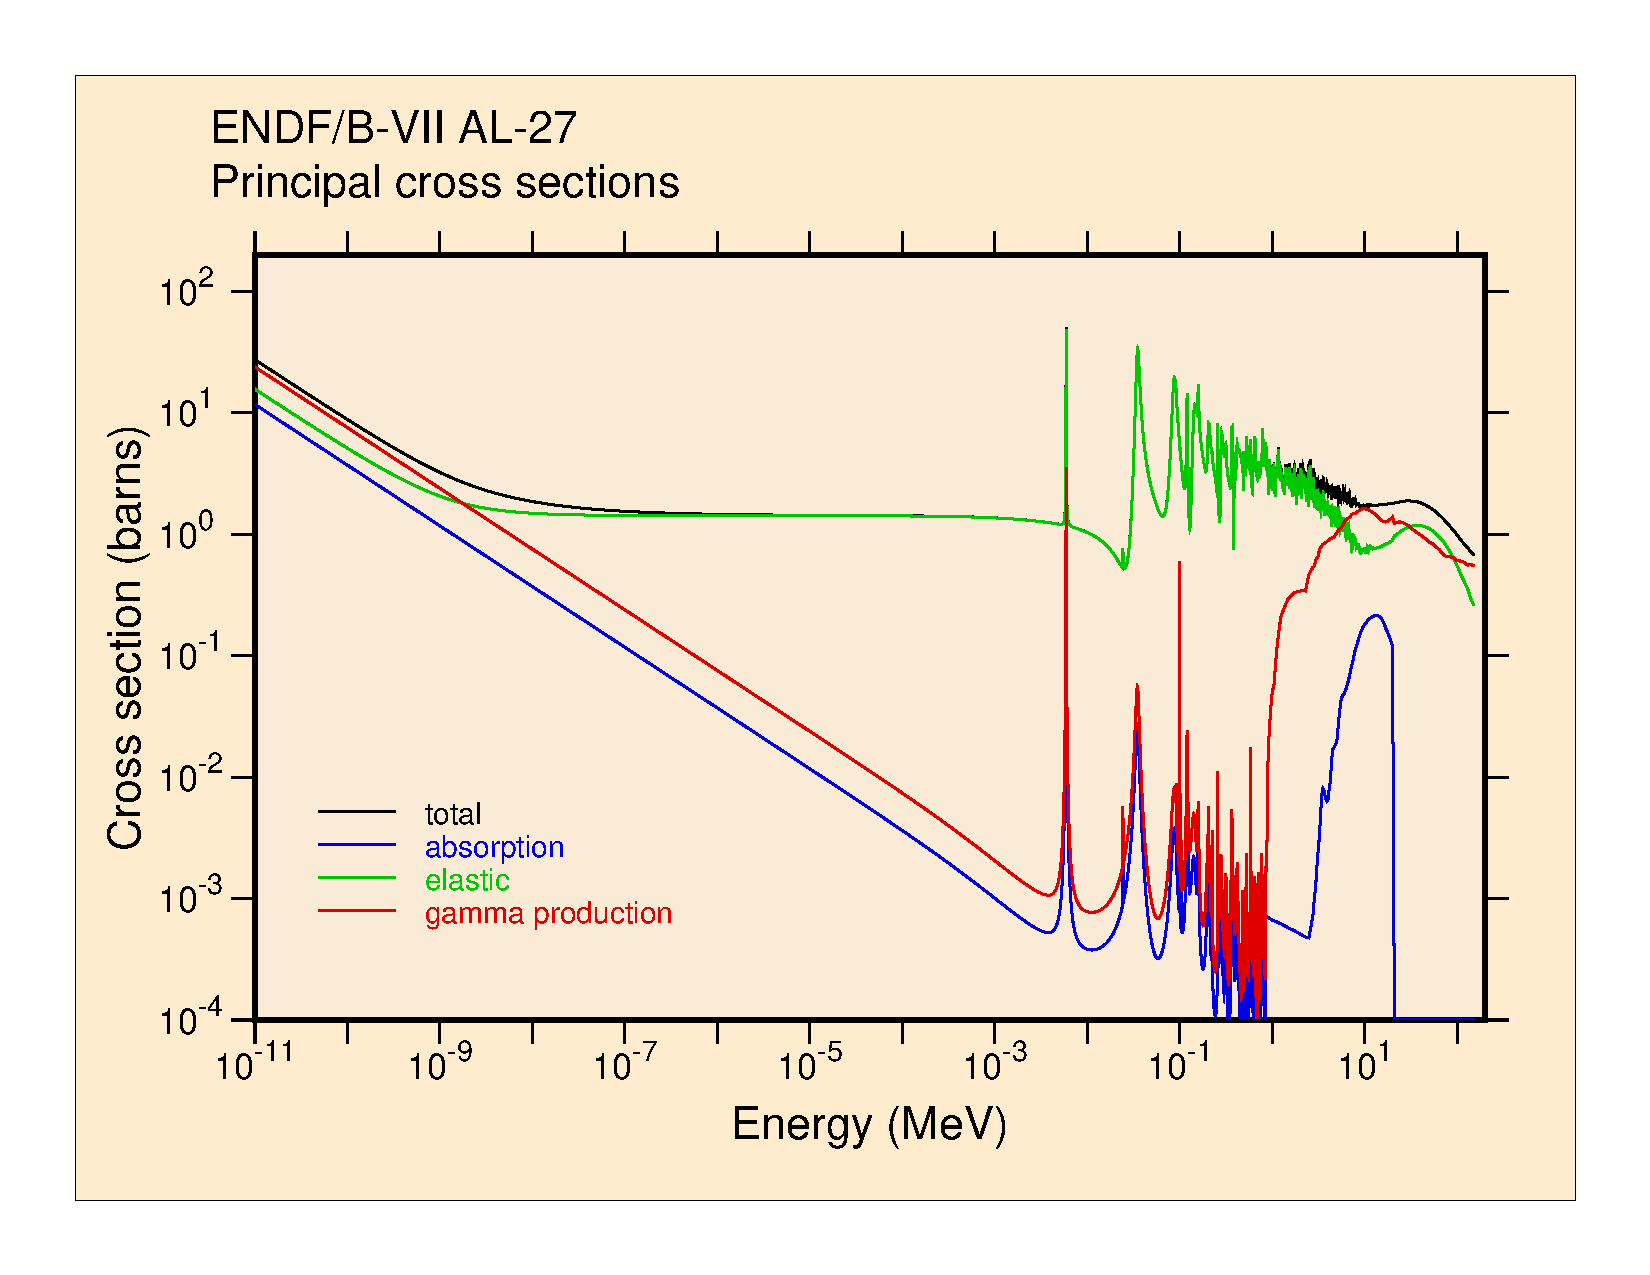
\includegraphics[keepaspectratio, height=4.0in, angle=0]{figs/acer1ack}
\caption[Principal cross sections for ENDF/B-VII.0 $^{27}$Al]{A log plot
 of the ACE principal cross sections for $^{27}$Al from ENDF/B-VII.0.  Note
 the extension beyond 20 MeV to 150 MeV.}
\label{pxsec}
\end{figure}

\begin{figure}[t]\centering
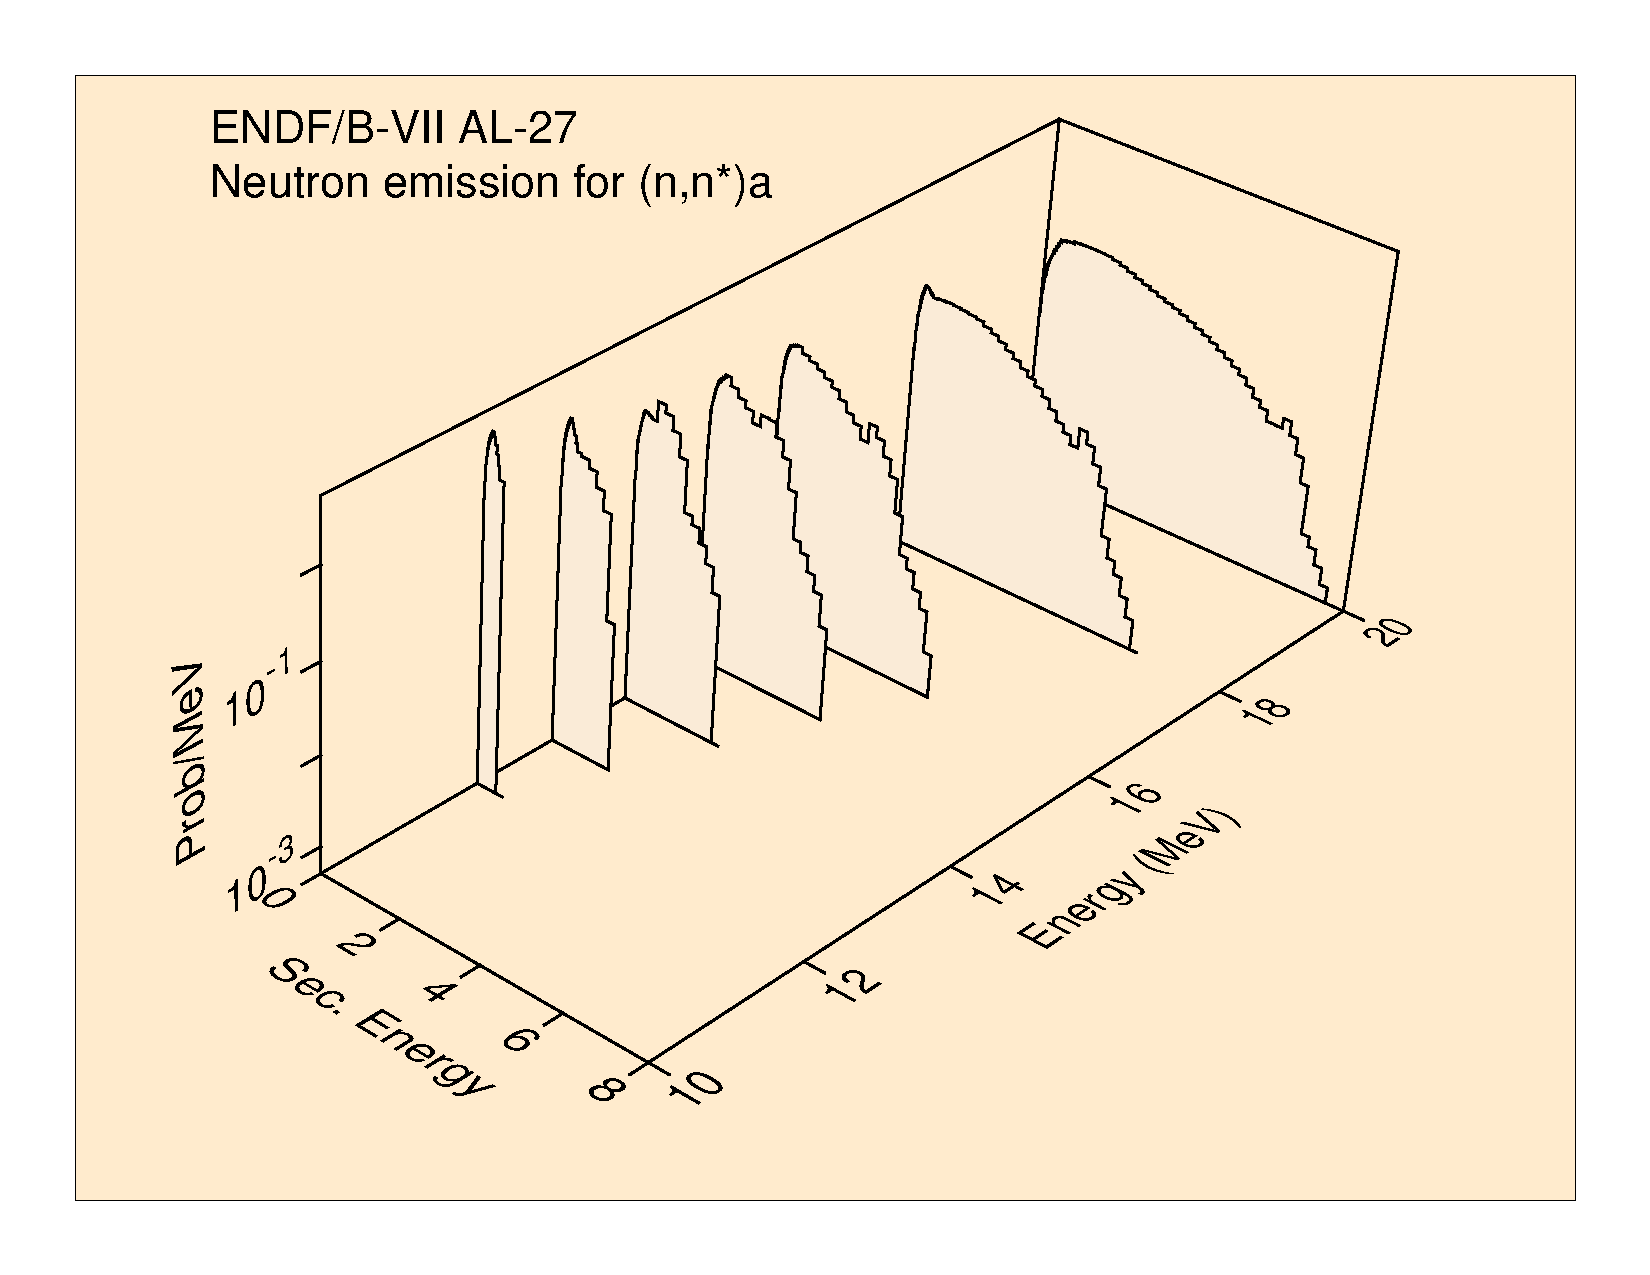
\includegraphics[keepaspectratio, height=3.6in, angle=0]{figs/acer2ack}
\caption[Neutron energy distributions from $^{27}$Al(n,n'$\alpha$)
 reaction]{A 3-D
 view of the energy distribution for neutrons emitted from the (n,n$'\alpha$)
 reaction on $^{27}$Al from ENDF/B-VII.}
\label{dist3d}
\end{figure}

\subsection{Thermal Cross Sections}
\label{ssACER_t}

Thermal data is the second class of ACE data to be considered,
\index{thermal cross sections}
and they are handled by the \cword{aceth}\index{modules!aceth@{\ty aceth}}
module.  This module exports two subroutines:
\cword{acesix}\index{acesix@{\ty acesix}} to process the data into
ACE format, and \cword{thrfix}\index{thrfix@{\ty thrfix}} for edits,
listings, and plots.

For energies below several eV, the thermal motions of nuclei can
lead to significant energy gains in neutron scattering.  In addition,
the binding of atoms into liquids and solids begins to affect the
scattering cross section and the distribution of scattered neutrons
in angle and energy.  MCNP can handle thermal neutron scattering
from the atoms of a free gas\index{free gas} using internal
kinematic formulas that assume a Boltzmann distribution.
The bound-atom effects are treated using thermal data from ENDF
evaluations stored in a special MCNP thermal library.

The ENDF format allows for several thermal processes.  Thermal
inelastic\index{thermal inelastic} scattering is represented using
the scattering law $S(\alpha,\beta)$\index{$S(\alpha,\beta)$}, where
$\alpha$ and $\beta$ are dimensionless momentum and energy transfer
parameters, respectively:

\begin{equation}
  \sigma(E{\rightarrow}E',\mu)=\frac{\sigma_{\rm b}}
   {4\pi T}\sqrt{\frac{E'}{E}}{\rm e}^{-\beta/2}S(\alpha,\beta)\,\,,
\end{equation}
\vspace{0.5 pt}

\noindent
where
\begin{equation}
  \alpha=\frac{E'+E-2\mu\sqrt{EE'}}{AkT}\,\,,
\end{equation}
\vspace{0.5 pt}

\noindent and
%\hbox{ }
\begin{equation}
  \beta=\frac{E'-E}{kT}\,\,.
\end{equation}
\vspace{0.5 pt}

\noindent
$E$ and $E'$ are the incident and outgoing neutron
energies, $\mu$ is the scattering cosine, $T$ is the absolute
temperature, $A$ is the mass ratio to the neutron of the
scatterer, and $k$ is Boltzmann's constant.  This process
occurs in all the ENDF thermal materials, such as water,
heavy water, graphite, beryllium, beryllium oxide, polyethylene,
benzine, and zirconium hydride.
\index{water}
\index{heavy water}
\index{graphite}
\index{Be}
\index{BeO}
\index{polyethylene}
\index{benzine}
\index{zirconium hydride}

The \hyperlink{sTHERMRhy}{THERMR}\index{THERMR}
module of NJOY uses this equation and evaluated
$S(\alpha,\beta)$\index{$S(\alpha,\beta)$} data from an ENDF-format
evaluation to compute $\sigma(E{\rightarrow}E',\mu)$.  The $E'$ dependence
of the integral over $\mu$ is computed adaptively so as to
represent the function using linear interpolation within a
specified tolerance.  The angular distribution at each of
these $E'$ values is then calculated in a similar way, but
the curve of $\sigma$ vs. $\mu$ is then converted into
equally probable bins (typically 8), and a discrete angle is
selected for each bin that preserves the average scattering
cosine for that bin.  The data are written onto the PENDF
tape using special MF=6-like formats.

The \cword{acesix}\index{acesix@{\ty acesix}} subroutine reads this
thermal section on the input PENDF\index{PENDF} file.  In older
versions of this method, the energy distribution
$\sigma(E\rightarrow E')$ is converted into equally probable bins
(typically 16), and a discrete energy is chosen for each bin that
preserves the average energy in that bin.  The result of this process
is a set of equally probable events\index{equally probable events}
(typically $8\times 16=128$ events) in $E',\mu$ space for each
incident energy.  It is very easy to sample from this representation,
and it is fairly compact.  See \cword{iwt}=0 is the input
instructions.

However, it must be recognized that this scheme is only reasonable
if each neutron undergoes several scattering events before being
detected.  The artificial discrete lines must be averaged out.  Be
careful when using this method to analyze experimental arrangements
using optically thin elements and small-angle detectors.  In addition,
as in all equal-probability bin schemes, the wings of functions
(which may be unlikely but important) are not well sampled.  ACER
includes a variation to partially relieve this problem: instead of
equal bin weights, the pattern 1, 4, 10, 10,..., 10, 4, 1 is used
(see ``variable weighting'' in the input instructions).  This approach
produces some samples fairly far out on the wings of the energy
distribution.  Angles are still equally weighted.  See \cword{iwt}=1
in the input instructions.

In practice, this method using discrete energies can still leave
some artificial peaks in typical thermal neutron spectra.  These
peaks don't have much effect on average quantities for most
applications, but they are visually offensive.  The newer versions
of MCNP (version 5.1.50 and later) support continuous distributions
of $\sigma(E\rightarrow E')$ with PDF and CDF values to drive the
sampling.  See \cword{iwt}=2 in the input instructions.  This is
the preferred representation.  The thermal inelastic data prepared by
\cword{acesix}\index{acesix@{\ty acesix}} is loaded into the ACE blocks
ITIE and ITXE by \cword{thrlod}\index{thrlod@{\ty thrlod}}.

The second ENDF process to consider is ``coherent elastic'' scattering.
\index{coherent elastic} This process occurs in powdered crystalline
materials, such as graphite, beryllium, and beryllium oxide.  Bragg
scattering from the crystal planes leads to jumps in the cross
section vs. energy curve\index{Bragg edges} as scattering from each
new set of planes becomes possible.  The formula for this process can
be written in the following form:

\begin{equation}
   \sigma(E,\mu)=\sigma_{\rm c}
    \frac{\pi\hbar^2}{4MEV}
     \sum_{\tau\ne 0}^{\tau<\tau_{\rm max}}
      f(\tau)\delta(\mu-\mu_0[\tau])\,\,,
\end{equation}

\noindent
where

\begin{equation}
   \tau_{\rm max}=\sqrt{\frac{8ME}{\hbar^2}}\,\,,
\end{equation}

\noindent
and

\begin{equation}
   \mu_0=1-\frac{\hbar^2\tau^2}{4ME}\,\,,
\end{equation}

\noindent
and where $E$ is the incident neutron energy, $E'$ is the outgoing
neutron energy, $\mu$ is the scattering cosine, $\sigma_{\rm c}$ is
the characteristic coherent scattering cross section
\index{coherent cross section} for the material, $M$ is the target
mass, $V$ is the volume of the unit cell, $\tau$ is the radius
of one of the reciprocal lattice shells, and $f(\tau)$ is the
effective structure factor for that shell.

Examination of these equations shows that the angle-integrated
cross section will go through a jump proportional to $f(\mu)$ when
$E$ gets large enough so that $\mu_0=-1$ for a given value of $\tau$.
At this energy, a backward directed component of discrete-angle
scattering will appear.  As the energy increases, this discrete-angle
line will shift toward the forward direction.  It is clear that the
only information that MCNP needs to represent this process in
complete detail is a histogram $P(E)$ tabulated at the values of $E$
where the cross section jumps.  The cross section will then be given
by $P(E)/E$.  The intensity and angle of each of the discrete lines
can be deduced from the sizes of the steps in $P(E)$ and the $E$
values where the steps take place.

The $P(E)$ function is computed from $\sigma(E)$ in \cword{acesix}.
Subroutine \cword{thrlod} stores the number of Bragg edges, the Bragg
energies, and the $P$ values at the Bragg edges into the ACE-format
ITCE block.

The third ENDF thermal process is incoherent elastic scattering.
\index{incoherent elastic}
\index{polyethylene}
\index{zirconium hydride}
It occurs for hydrogenous solids like polyethylene and
zirconium hydride by virtue of the large incoherent scattering length
and small coherent scattering length of hydrogen.  The equation
describing this process is

\begin{equation}
  \sigma(E,\mu)=\frac{\sigma_{\rm b}}{2}
   {\rm e}^{-2EW(1-\mu)/A}\,\,,
\end{equation}

\noindent
where $\sigma_{\rm b}$ is the characteristic bound cross section, and
$W$ is the Debye-Waller integral.  The \hyperlink{sTHERMRhy}{THERMR}
module\index{THERMR} of NJOY computes the integrated cross
section $\sigma(E)$ for this process and a set of equally
probable cosines\index{equally probably cosines}
for each incident energy $E$; it writes them onto the PENDF tape using
a special format.  These quantities are copied into the ITCE and ITCA
blocks of the ACE format in subroutine \cword{thrlod}.

No consistency checking is currently available for thermal files,
but a set of plots is provided to help with QA.
\index{ACER quality assurance}  The plots are prepared as input
for the \hyperlink{sVIEWRhy}{VIEWR} module, which can generate the
final color Postscript files for plotting.  A log plot of the
total, inelastic, and elastic (if present) cross sections is
given first, followed by by plots of the average scattering cosine,
mubar, and the average energy of the scattering neutrons, ebar.
Perspective views of the energy spectrum for thermal neutron
scattering are provided, and several plots of the angle-energy
emission for different incident energies are also present.
Fig.~\ref{hh2o-ae} shows an example of an angular distribution plot.

\begin{figure}[thb]\centering
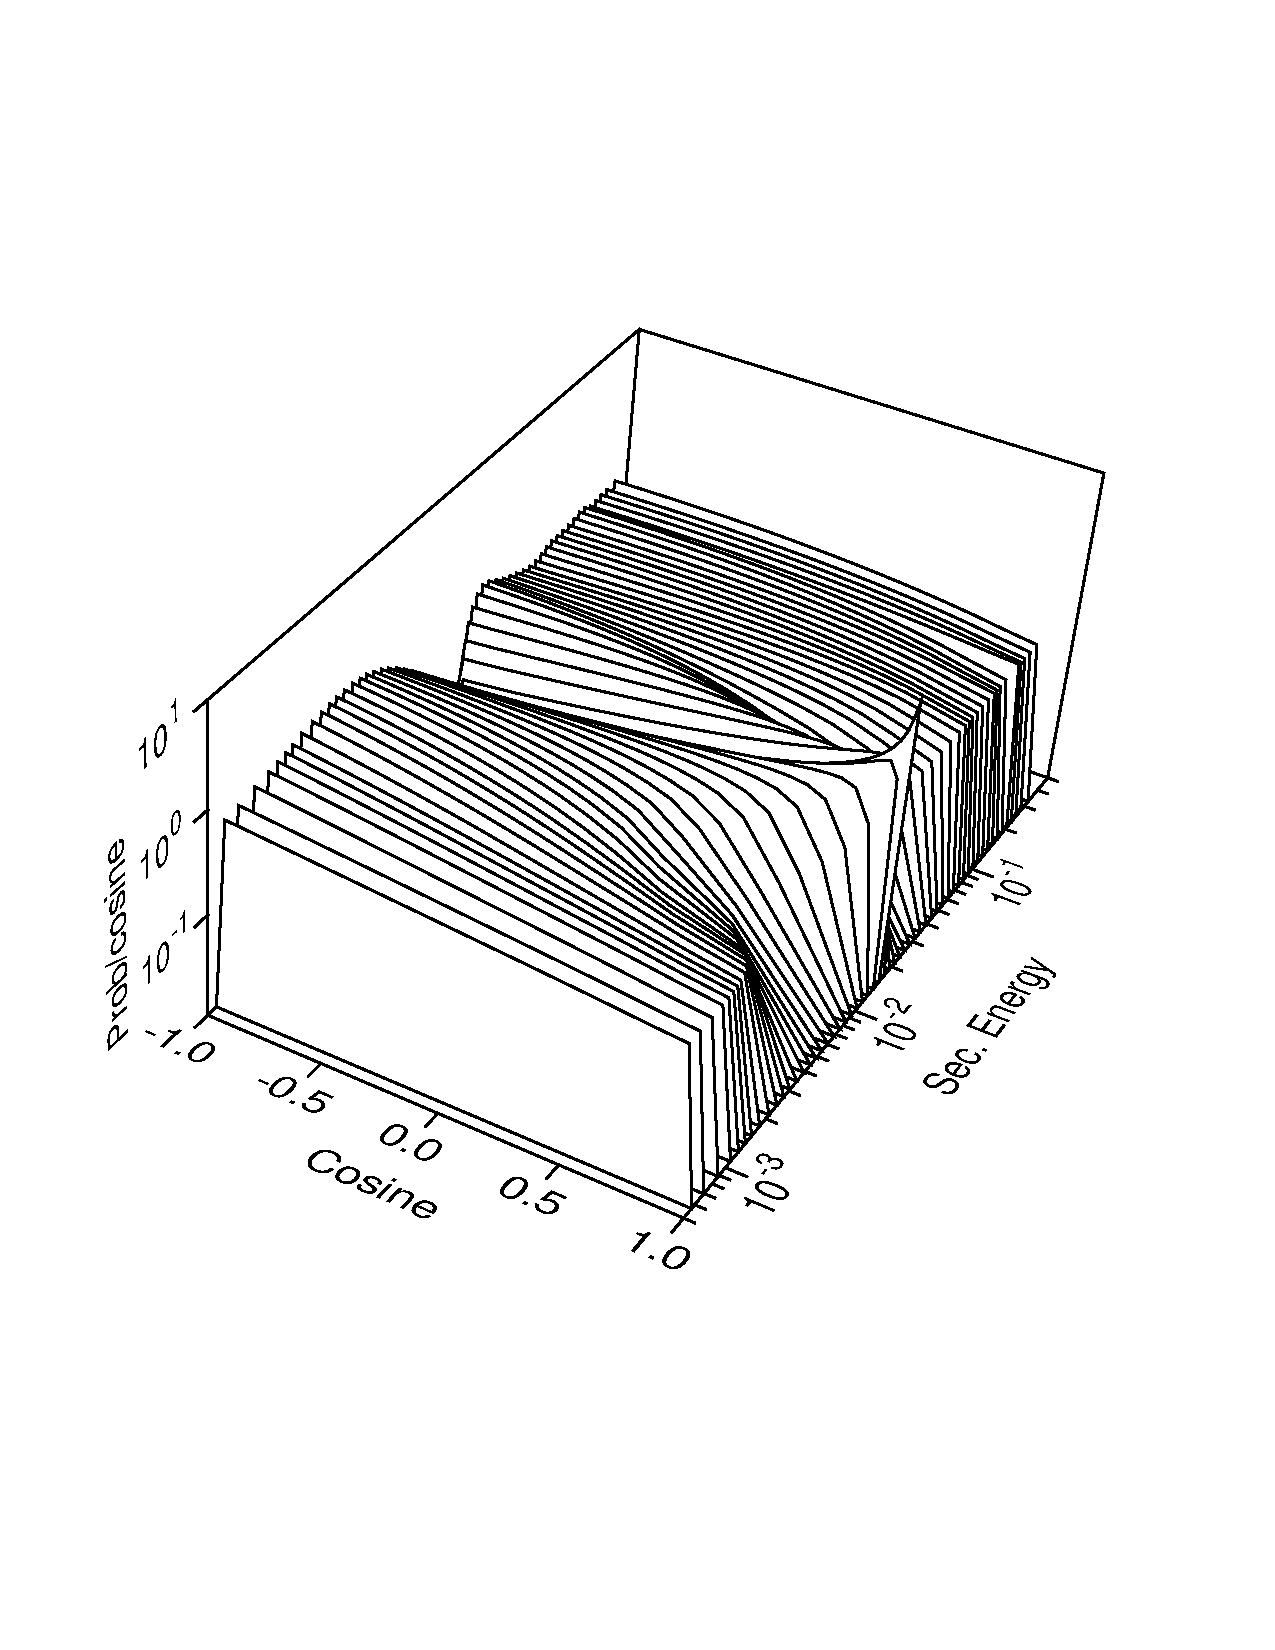
\includegraphics[keepaspectratio, height=4.0in, angle=0]{figs/hh2o-aeack}
\caption[Neutron scattering distribution from H in H$_2$O]{A perspective
 view of an angle-energy distribution for H in H$_2$O.}
\label{hh2o-ae}
\end{figure}


\subsection{Dosimetry Cross Sections}
\label{ssACER_dosimetry}

The ACE dosimetry\index{dosimetry} data forms another class
of MCNP data, and they are handled by the
\cword{acedo}\index{modules!acedo@{\ty acedo}} sub-module of the
ACER group. This class of library provides cross sections to be
used for response functions in MCNP; the data cannot be used
for actual neutron transport.  The information on a dosimetry file
is limited to an MTR block, which describes the reactions
included in the set, an LSIG block containing pointers to the
cross section data for the reactions, and the SIGD block,
which contains the actual data.  The format for dosimetry cross section
storage is different from the format for neutron cross sections.
The union grid for linear interpolation is not used; instead, the
cross sections are stored with their ENDF interpolation laws.  If
the file mounted as the input PENDF tape is a real PENDF tape (that is,
if it has been through \hyperlink{sRECONRhy}{RECONR}),
all the reactions are already linearized,
and the interpolation information stored in the SIGD block will
indicate linear interpolation for a single interpolation
range.  However, if the file mounted as NPEND is actually an ENDF
file, the SIGD block may indicate multiple interpolation ranges with
nonlinear interpolation laws.

\subsection{Photoatomic Data}
\label{ssACER_pa}

Photoatomic data\index{photoatomic} form another ACE class.
The data are processed using the \cword{acepa}
\index{modules!acepa@{\ty acepa}}module, which exports
the subroutine \cword{acepho}\index{acepho@{\ty acepho}} for
formatting the data, and the subroutine
\cword{phofix}\index{phofix@{\ty phofix}} for editing, listing,
consistency checks, and plots.

Photons from direct sources and photons produced by neutron reactions
are scattered and absorbed by atomic processes, producing heat at the
same time.  The existing MCNP ``photon interaction'' libraries were
based on fairly old cross section data and assembled by
hand\cite{MCG,MCP}.  This version of ACER contains the beginnings
of an automated capability to produce these libraries from the latest
ENDF/B photoatomic data.\index{photon interaction cross sections}

The cross sections for the basic photoatomic process incoherent
scattering, coherent scattering, pair production, and photoelectric
absorption are given on a union energy grid.  Actually, the energies
and the cross sections are stored as logarithms, and MCNP uses
linear interpolation on them; therefore, the effective interpolation
law is log-log.  MCNP determines the mean-free-path to a reaction
using the sum of these partial cross sections instead of a total
cross section.
\index{photoatomic!pair production}
\index{photoatomic!photoelectric}
\index{photoatomic!coherent}
\index{photoatomic!incoherent}

If the reaction is incoherent (Compton) scattering, the scattering
is assumed to be given by the product of the free-electron
Klein-Nishina cross section and the incoherent scattering function,
\index{Klein-Nishina}
$I(v)$.  MCNP assumes that this function is tabulated on a given
21-point grid of $v$ values, where $v$ is the momentum of the recoil
electron given in inverse angstroms.  It is easy to extract the
scattering function from the section MF=26, MT=504 of the photoatomic
ENDF library and to interpolate the function onto the required $v$
grid.

If the reaction is coherent (Thomson) scattering, the photon will
be scattered without energy loss, and the scattering distribution is
given by the Thomson cross section times the coherent form factor.
\index{Thomson cross section}
\index{atomic form factors}
The sampling scheme used in MCNP requires the coherent form factor
tabulated on a predefined set of 55 $v$ values, and it also requires
integrated form factors tabulated at 55 values of $v^2$, where the
$v$ values are the same set used for the form factors.  These values
are extracted from the section MF=26, MT=502, and the integrals are
done using the standard NJOY routine \cword{intega}.
\index{intega@{\ty intega}}

Photoelectric absorption results in the emission of a complex pattern
of discrete ``fluorescence''\index{fluorescence} photons and electrons
(which lead to heating) due to the cascades through the atomic levels
as the atom de-excites.

The fluorescence part is not coded yet.  This section will be
completed when the new fluorescence methods have been developed and
installed in MCNP.  In the meantime, ambitious users may be able
to meld the new cross sections computed by the methods discussed
in this section with the fluorescence data from the current MCNP
library.


\subsection{Photonuclear Data}
\label{ssACER_pn}

Photonuclear data\index{photonuclear data} forms a new class of
ACE data that has just become available in recent years.
These data are handled by the module
\cword{acepn}\index{modules!acepn@{\ty acepn}},
which exports the call \cword{acephn}\index{acephn@{\ty acephn}}
for processing the data into ACE format, and the call
\cword{phnfix}\index{phnfix@{\ty phnfix}} for editing, listing,
consistency checks, and plots.  A fairly large number of
photonuclear evaluations is available as of this writing.  They were
originally collected by the Data Section of the IAEA\index{IAEA},
and they then migrated into ENDF/B-VII.0.

The new ACE photonuclear format differs in some ways from the
more familiar continuous-energy format (class ``c'').  In this format,
all emissions (neutrons, photons, and charged particles) are
treated symmetrically using blocks with the style of the particle
production blocks from the class ``c'' format.  Each possible
reaction product is described by a production cross section,
a partial heating value, fractions represented by different
reaction channels, and angle, energy, or energy-angle distributions
for each reaction channel.

One class of the new evaluations consists of those performed at
LANL\index{Los Alamos National Laboratory!LANL} and a large set of materials
using the same methods generated at the Korea Atomic Energy Research
Institute (KAERI)\index{KAERI}.  These evaluations lump all the
photonuclear processes into a single reaction with MT=5 and use
subsections of MF=6/MT=5 to represent all the neutrons, photons,
and charged particles produced.  These are processed by using the
energy grid of MT=5 as the union grid.  The ACE total and heating
values are constructed on this grid.  Then the sections of File 6
are processed to generate production cross sections and partial
heating values for each of the emitted species.  Each emitted
neutron or charged particle also has an energy-angle
distribution associated with it, represented using the Kalbach LAW=44
format, and emitted photons are represented using LAW=4.


\subsection{Type 1 and Type 2}
\label{ssACER_ty12}

ACE library files come in two different types in order to allow
for efficiency and portability.
\begin{itemize}
\begin{singlespace}
\item Type 1 is a simple formatted file suitable for
       exchanging ACE libraries between different computers.

\item Type 2 is a FORTRAN-77 direct-access binary file
       for efficient use during actual MCNP runs.
\end{singlespace}
\end{itemize}
\vspace{3 pt}

\noindent
There used to be Type 3 using word-addressable random access
methods, but these methods were machine specific, and the
type has been abandoned.
\index{ACE format!Type 1}
\index{ACE format!Type 2}
\index{ACE format!Type 3}
ACER stores all values in memory as real numbers, and it is easy
to write them out in Type-2 format, because all fields in that format
are also represented by real numbers (except for some of the fields
in the header record).  The Type 1 format requires that fields
that represent integers must be written in integer format,
that is, right justified and without decimal points.
The output routines in the ACER submodules contain logic to
perform this step (see \cword{aceout}, \cword{throut}, \cword{dosout},
\cword{phoout}, and \cword{phnout}).
\index{throut@{\ty throut}}
\index{dosout@{\ty dosout}}
\index{phoout@{\ty phoout}}
\index{phnout@{\ty phnout}}

The ACER user can prepare libraries using either Type 1 or Type 2
output.  The advantage of Type 1 is that the files can be easily moved
to other machines or laboratories.  The advantage of Type 2 is that
it is more compact and can be used directly by MCNP with no performance
penalties.  At any time, ACER can be used to convert one format to
another, or to make a listing of the data from any of the formats (see
\cword{iopt} values from 7 through 9 in the input instructions).

\subsection{Running ACER}
\label{ssACER_running}

The following input instructions are copied from the comment
cards at the beginning of the ACER module.  Users
should always check the actual comment cards for the current
version to see if there have been any changes.
\index{ACER!ACER input}
\index{input!ACER}

\small
\begin{ccode}

   !---input specifications (free format)---------------------------
   !
   ! card 1
   !    nendf    unit for input endf tape
   !    npend    unit for input pendf tape
   !    ngend    unit for input multigroup photon data
   !    nace     unit for output ace tape
   !    ndir     unit for output mcnp directory
   ! card 2
   !    iopt     type of acer run option
   !               1   fast data
   !               2   thermal data
   !               3   dosimetry data
   !               4   photo-atomic data
   !               5   photo-nuclear data
   !               7   read type 1 ace files to print or edit
   !               8   read type 2 ace files to print or edit
   !                set iopt negative for mcnpx format
   !    iprint   print control (0 min, 1 max, default=1)
   !    itype    ace output type (1, 2, or 3, default=1)
   !    suff     id suffix for zaid (default=.00)
   !    nxtra    number of iz,aw pairs to read in (default=0)
   ! card 3
   !    hk       descriptive character string (70 char max)
   !             delimited by quotes
   ! card 4 (nxtra.gt.0 only)
   !    iz,aw    nxtra pairs of iz and aw
   !
   !    --- fast data (iopt=1 only) ---
   !
   ! card 5
   !    matd     material to be processed
   !    tempd    temperature desired (kelvin) (default=300)
   ! card 6
   !    newfor   use new cumulative angle distributions,
   !               law 61, and outgoing particle distributions.
   !               (0=no, 1=yes, default=1)
   !    iopp     detailed photons (0=no, 1=yes, default=1)
   !    ismooth  switch on/off smoothing operation (1/0, default=1=on)
   !               set ismooth to 1 to cause extension of mf6 cm
   !               distributions to lower energies using a sqrt(E)
   !               shape, to extend delayed neutron distributions as
   !               sqrt(E) to lower energies, and to add additional
   !               points above 10 Mev to some fission spectra assuming
   !               an exponential shape.  otherwise, use ismooth=0.
   !               NOTE:  ismooth=0 is the default value in njoy99.
   ! card 7
   !  type of thinning is determined by sign of thin(1)
   !  (pos. or zero/neg.=energy skip/integral fraction)
   !  (all entries defaulted=no thinning)
   !    thin(1)  e1 energy below which to use all energies (ev)
   !             or iwtt weighting option (1=flat,2=1/e)
   !             (1/e actually has weight=10 when e lt .1)
   !    thin(2)  e2 energy above which to use all energies
   !             or target number of points
   !    thin(3)  iskf skip factor--use every iskf-th energy
   !             between e1 and e2, or rsigz reference sigma zero
   !
   !   --- thermal data (iopt=2 only) ---
   !
   ! card 8
   !    matd     material to be processed
   !    tempd    temperature desired (kelvin) (default=300)
   !    tname    thermal zaid name ( 6 char max, def=za)
   ! card 8a
   !    iza01    moderator component za value
   !    iza02    moderator component za value (def=0)
   !    iza03    moderator component za value (def=0)
   ! card 9
   !    mti      mt for thermal incoherent data
   !    nbint    number of bins for incoherent scattering
   !    mte      mt for thermal elastic data
   !    ielas    0/1=coherent/incoherent elastic
   !    nmix     number of atom types in mixed moderator
   !             (default=1, not mixed)
   !             (example, 2 for beo or c6h6)
   !    emax     maximum energy for thermal treatment (ev)
   !             (default=1000.=determined from mf3, mti)
   !    iwt      weighting option
   !             0/1/2=variable/constant/tabulated (default=variable)
   !
   !   --- dosimetry data (iopt=3 only) ---
   !
   ! card 10
   !    matd     material to be processed
   !    tempd    temperature desired (kelvin) (default=300)
   !
   !   --- photo-atomic data (iopt=4 only) ---
   !
   ! card 11
   !    matd     material to be processed
   !             photoatomic data on nendf
   !             atomic relaxation data on npend
   !
   !   --- photo-nuclear data (iopt=5 only) ---
   !
   ! card 12
   !    matd     material to be processed
   !
   !   --- print or edit existing files (iopt=7-9) ---
   !
   !    No additional input cards are required.  Mount the old
   !    ace tape on "npend".  The code can modify zaid, hk,
   !    the (iz,aw) list, and the type of the file.  Use suff<0
   !    to leave the old zaid unchanged.  Use just "/" on
   !    card 3 to leave the comment field hk unchanged.  Use
   !    nxtra=0 to leave the old iz,aw list unchanged.  The
   !    code can modify zaid, hk, and type of file.
   !
   !    Exhaustive consistency checks are automatically made on
   !    the input file.  If ngend.ne.0, a set of standard ACE plots
   !    are prepared on unit ngend as plotr input instructions.
   !
   !--------------------------------------------------------------------

\end{ccode}
\normalsize

\paragraph{Card 1.}
ACER uses the information from the ENDF tape mounted on unit
\cword{nendf} for angle, energy, energy-angle, and photon emission
distributions, and it uses the data on \cword{npend} for the unionized
and linearized cross sections.  The latter file should have been
processed through \hyperlink{sRECONRhy}{RECONR}, and maybe
\hyperlink{sBROADRhy}{BROADR}.  If it wasn't, ACER will
still work, but the energy grids may not be quite right.  The
\cword{ngend} unit is only needed for input if the old 30$\times$20
photon production matrix is to be constructed; otherwise, set it to zero.
In addition, \cword{ngend} is used for plotting output (if available)
when one of the print or edit options is selected
(see \cword{iopt}=7 below; set it to zero to suppress plotting output.
Unit \cword{nace} is the main output tape for the ACE-format library, and
unit \cword{ndir} will contain a single line of text intended to be
edited and incorporated into a directory for a big multi-material ACE
library.

\paragraph{Card 2.}
The value of \cword{iopt} specifies the kind of ACE data being produced,
as indicated in the instructions.  The long print option, \cword{iprint}=1,
produces a complete, interpreted listing of the ACE data.  The shorter
print options just put out progress information from the ACER job and
a brief listing of the header information for the library that was
generated.  The \cword{ntype} parameter specifies whether the output
library will be in ASCII or binary form.  In MCNP jobs, materials are
identified by their ``zaid'' numbers (rhymes with ``staid''); they are
constructed by using the value 1000$\times$Z$+$A, appending the value
of \cword{suff} (the suffix), and then adding a letter that indicates
the library class (``c'' for continuous, ``t'' for thermal, {\it etc.}
(see Table~\ref{classes}).  For example, 92235.70c denotes a
continuous (fast data) library entry for $^{235}$U from ENDF/B-VII.
Thermal zaids are actually alphanumeric before the dot; see Card 8.
Finally, \cword{nxtra} is the number of extra \cword{iz}, \cword{aw}
pairs of values to be read in on Card 4.

\paragraph{Card 3.}
This card contains a descriptive character string up to 70 characters
long.  It must be delimited by ' characters and terminated by the /
character.

\paragraph{Card 4.}
Read in \cword{nxtra} pairs of numbers \cword{iz} and \cword{aw} for
photoatomic data.  Use as many cards as necessary.

\paragraph{Card 5.}
This is the first card for a fast data library run.  It specifies the
ENDF MAT number and the absolute temperature for the material to be
processed.   ENDF MAT numbers are 4-digit numbers.  For the earlier
versions of ENDF/B, they were assigned in an arbitrary way; for example,
1276 was $^{16}$O for ENDF/B-IV and 1395 represented $^{235}$U for ENDF/B-V.
For ENDF/B-VI and later, a systematic scheme has been selected that allows the
same MAT number to be used for all the various sub-libraries (for example,
neutron data, thermal data, incident proton data, {\it etc.}).  This
scheme is based on using Z to get the first two digits.  The second two
digits are chosen to be zero for elements, and for normal isotopes, they
step in units of 3 up and down around 25, the value for the lowest
isotope of the normal stable group of isotopes.  This leaves room for
two isomers for each isotope in between.  Examples include 9225 for
$^{234}$U, 9228 for $^{235}$U, and 2200 for natural Ti. If the
temperature is greater than zero, the input PENDF tape must have
been run through \hyperlink{sBROADRhy}{BROADR}.

\paragraph{Card 6.}
The flag \cword{newfor} is equal to 1 if the new cumulative
format for angular distributions, the LAW=61 format for energy-angle
data, and the particle production sections are desired; otherwise, it
is zero.  The default is \cword{newfor}=1, suitable for use with MCNP4C
and subsequent versions.  The flag \cword{iopp} determines whether the
newer detailed photon data option is used (preferred), or whether the
older 30$\times$20 photon production matrices are to be generated.
Remember that if the latter option is selected,
\hyperlink{sGROUPRhy}{GROUPR} must be run
before ACER to generate multigroup versions of the photon production
matrices for all reactions, and the resulting GENDF tape must be
coupled to ACER using the \cword{ngend} input parameter.

\paragraph{Card 7.}
Thinning of the union energy grid can be performed using several options
as described in detail in Section~\ref{ssACER_classes} above.  Defaulting
the entire card
by entering only / results in no thinning.  This is preferred.

\paragraph{Card 8.}
This card starts the input of parameters for the thermal library option.
The material MAT number and absolute temperature are given. The default
temperature is 293.6K and the default \cword{tname} is generated from ZA.
Therefore, the simplest version of this card would consist of a MAT
number followed by /.  Check the discussion above for Card 5.  In almost
all cases, an entry for \cword{tname} is desirable.  Examples are
``LWTR'' for H in light water (or ``HH2O'' for hydrogen in water),
``GRAPH'' for graphite, ``ZRZRH'' for zirconium in zirconium hydride,
and so on.

\paragraph{Card 8a.}
MCNP needs to know the zaid values to get the fast data needed to go
with a particular set of thermal data.  For a thermal set like HH2O,
only \cword{iza01}=1001 would be needed.  For a mixed moderator like
benzine, values for both \cword{iza01} and \cword{iza02} must
be given ({\it e.g}., 1001 and 6000).  See \cword{nmix} below.    The
third input parameter allows for the aliases 6012 and 6000, if
needed.

\paragraph{Card 9.}
The value \cword{mti} must correspond to one of the values used for
this material in the \hyperlink{sTHERMRhy}{THERMR} runs that
generated the input PENDF tape
(see Table~\ref{mti}).  The number of bins to use for the equally
probable bins for the outgoing neutron spectra is defined by
\cword{nbint}; the default value is 16.  The parameter \cword{mte}
defaults to zero; a nonzero value is only needed for materials that
show elastic scattering (see Table~\ref{mti}).  The value \cword{ielas}
indicates whether this elastic scattering is coherent or incoherent.
In the ENDF/B thermal evaluations, some isotopes for mixtures are
represented like water, which describes the scattering from hydrogen
bound in water, and some are given like benzine, which describes the
scattering from the benzine molecule normalized to the hydrogen cross
section.  The parameter \cword{nmix} is used to tell ACER about this
effect.  For the existing ENDF/B evaluations, the user should use
\cword{nmix}=2 for benzine; the user should use \cword{nmix}=1
for all other materials.  The parameter \cword{emax} defines the
maximum energy to be used for the thermal scattering treatment.  This
value should be coordinated with the value of \cword{emax} in
\hyperlink{sTHERMRhy}{THERMR}.  A number
around 4 eV is reasonable for most problems.  The default
for this parameter is 1000., which means that the code will determine
the upper limit from the data in MF=3 on the PENDF tape.  Thus, the
value used in \hyperlink{sTHERMRhy}{THERMR} is passed
into ACER without the user having to
check it.  The last parameter on Card 9 is \cword{iwt}.  As described
in Section~\ref{ssACER_t}, the weighting pattern for probability bins for
emitted thermal neutrons can be flat (that is, equally probable bins),
or it can be variable in the pattern 1, 4, 10, 10,..., 10, 4, 1 in
order to better sample the outlying wings of the energy distribution.
The default is variable.  Better yet, for modern MCNP 5.1.50 and later,
use \cword{iwt}=2, which gives a continuous distribution in outgoing
energy, eliminating the discrete energy spikes.

The simplest version of Card 9 would contain only \cword{mti} followed
by /.  This works for many materials, including water, heavy water,
and benzine, but if an elastic (coherent or incoherent) component is
present than the appropriate \cword{mte} value must also appear.
\index{thermal MT numbers}

\begin{table}[thb]
\setlength{\extrarowheight}{1pt}
\caption[ENDF/B-VII thermal MT numbers used in ACER and THERMR]{Conventional
 values for the thermal MT numbers (\cword{MTI} and \cword{MTE}) used in ACER
 and \hyperlink{sTHERMRhy}{THERMR} for ENDF/B-VII}
\label{mti}
\begin{center}
\begin{tabular}{lll}
Thermal Material & \cword{MTI} Value & \cword{MTE} Value \\
\hline
H in H$_2$O & 222 &   \\
D in D$_2$O & 228 &   \\
Be metal & 231 & 232 \\
Graphite & 229 & 230 \\
Benzine  &  227  &  \\
Zr in ZrH & 235 & 236 \\
H in ZrH  &  225 & 226 \\
Be(BeO)  &  233 & 234 \\
O(BeO)  & 237 & 238 \\
H in Polyethylene & 223 & 224 \\
U(UO$_2$)  & 241 & 242 \\
O(UO$_2$) & 239 & 240 \\
Al  & 243 & 244 \\
Fe  &  245 & 246  \\
\hline
\end{tabular}
\end{center}
\end{table}

\paragraph{Card 10.}
This card is used for dosimetry libraries only.  It specifies the
material MAT number and absolute temperatures.  See the discussion
of \cword{mat} and \cword{tempd} for the fast (continuous) libraries.

\paragraph{Card 11.}
Photoatomic libraries require only the single parameter \cword{matd}.
For ENDF/B-VII input, this will be a number like 100 for hydrogen
or 9200 for uranium.

\paragraph{Card 12.}
Photonuclear libraries require only the single parameter \cword{matd}.
See the discussion of \cword{mat} for the fast (continuous) libraries.

\paragraph{Editing Runs.}
No special input cards are required for editing runs.  The class of data
in the library is automatically determined from the ZAID suffix.  The
type of the output library is determined by \cword{ntype} on Card 2.
Changes can be made in the fields \cword{zaid}, \cword{hk}, and in the
(\cword{iz,aw}) list.  One common use for these editing parameters would
be as follows.  A user runs several isotopes, one at a time, using the
default ZAID of ``.00c'', and 1/E integral thinning.  Later, the user
decides that all these materials  should go into a particular library
with the suffix ``.77c'' and the comment field ``ENDF/B-VII library 7
for thermal reactor applications.'' ACER can handle these changes.

The following is a typical ACER input deck for producing a
continuous-energy file (class ``c''):

\small
\begin{ccode}

      acer
      20 21 0 31 32/
      1 0 1/
      'ENDF/B-VII U-238'/
      9237 293.6/
      /
      /
      acer
      0 31 33 34 35/
      7 1 1/
      'ENDF/B-VII U-238'/
      viewr
      33 36/
      stop

\end{ccode}
\normalsize

\noindent
It assumes that the ENDF file for $^{238}$U from ENDF/B-VII has
been mounted on unit 20 (\cword{tape20}) and that the corresponding
PENDF tape (after running through \hyperlink{sRECONRhy}{RECONR},
\hyperlink{sBROADRhy}{BROADR}, {\it etc.}) has
been mounted on unit 21 (\cword{tape21}).  We have used \cword{iopt}=1
for fast continuous data, suppressed the output listing with
\cword{iprint}=1, and requested Type-1 output (\cword{itype}=1).
Any desired descriptive line may be used, but some library schemes
might like to define special arrangements of text.  The proper ENDF
MAT number for $^{238}$U is 9237, and we are taking the first temperature
produced in the \hyperlink{sBROADRhy}{BROADR} run,
namely, 293.6K.  This corresponds to
0.0253e-6 MeV, the standard base temperature for MCNP data files.
We have taken the default values for \cword{newfor} and \cword{iopp},
so we expect to see the new formats and the detailed photon data.
We have also taken the default of no thinning, which is preferred with
modern large computers.  The output ACE file and XSDIR line will
appears on \cword{tape31} and \cword{tape32}.  The second ACER run
is used to provide QA checks.  It reads in the Type-1 file from
\cword{tape31} and writes out a new Type-1 file and a new XSDIR
line on \cword{tape34} and \cword{tape35}, respectively.  While
doing this, it runs the consistency checks and makes a set of plots
on \cword{tape33}.  If the consistency plots find an $E'>E'_{max}$
error that can be repaired, the modified result will be on
\cword{tape34}.  Finally, the \hyperlink{sVIEWRhy}{VIEWR}
module is run to convert the
information on \cword{tape33} into color Postscript plots on
\cword{tape36}.  The actual step of reading the ACE file is a
useful QA step, as are the consistency checks and plots.  In addition,
it is good practice to run the output ACE file immediately into
an simple MCNP test job to see if it really scans correctly.  This
is easy to do by incorporating the input example above and the
MCNP test input into a single script.

The second input example for ACER is for producing a thermal
class ``t'' library for hydrogen in water at a temperature of
800K using continuous energy distributions:

\small
\begin{ccode}

       acer
       20 21 0 31 32/
       2 0/
       '1-h-1 in h2o at 800k from endf-vii'/
       125 800 'hh2o'/
       1001/
       222 64 0 0 2/
       acer
       0 31 22 33 34/
       7 1/
       '1-h-1 in h2o at 800k from endf-vii'/
       viewr
       22 23/
       stop

\end{ccode}
\normalsize

\noindent
Here we have the additional entry \cword{tname='hh2o'}, which is
used to construct the ZAID value (which will be ``hh2o.00t'').
We have used \cword{mti}=222, the standard value for hydrogen
in water (see Table~\ref{mti}) and requested 64 bins with
the continuous tabulated data the outgoing neutron spectrum.
Experience has shown that more bins than the default of 16 are often
desirable.


\subsection{Coding Details}
\label{ssACER_details}

ACER begins in the \cword{acer}\index{acer@{\ty acer}} routine
provided by module \cword{acem}\index{modules!acem@{\ty acem}}
by reading the user's input.  The input varies according to
whether ``fast'', ``thermal'', ``dosimetry'', ``photoatomic'',
or photonuclear'' data are wanted, or if editing or type conversion
is desired.  See \cword{iopt}.  For regular processing runs
(\cword{iopt}=1-5), input ENDF and PENDF\index{PENDF} tapes are required,
the input GENDF tape is only needed if a photon production
matrix is to be constructed.  For edit runs, the input
ACE file is mounted on the PENDF unit, and the GENDF unit is used
for plotting output, if desired.  The code then branches to a
different subroutine (in a different module) for each different value
of \cword{iopt}.

Processing of fast data is controlled by \cword{acetop}
\index{acetop@{\ty acetop}} (which is in the
\cword{acefc} module\index{modules!acefc@{\ty acefc}}).
It begins begins by opening the ENDF, PENDF, and GENDF units, and
by opening a scratch file MSCR used to accumulate the input for
the \cword{acelod}\index{acelod@{\ty acelod}} procedure.  Subroutine
\cword{first}\index{first@{\ty first}} is then called to read
the MF=1 and MF=2 data from the input tapes and to prepare
the corresponding data on MSCR.  It copies the TAPEID record
and Hollerith descriptive data on the PENDF tape to MSCR, and it
processes the directory on the ENDF tape in order to set flags that
depend on which reactions and data types are present.  For example,
\cword{mt19} is set if a distribution is provided for MT=19, in
addition or instead of the more standard MT=18.  The global variables
\cword{nf12s}, \cword{mf1x}, and \cword{gmt} are used to keep track
of the reactions involved in computing photon production.  For the
new format (\cword{newfor}=1), the MT=3 reactions that imply the
production of neutrons or charged particles (either directly or as a
residual) are identified.  The MF, MT, and product identity for each
such reaction is stored in the arrays \cword{kprod}, \cword{mprod},
and \cword{iprod}, respectively, for a total of \cword{nprod} items.
Subroutine \cword{first} continues by standardizing and copying the
fission neutron yield sections (see \cword{tabize}), by writing a
dummy File 2 on \cword{mscr}, and by copying the probability tables
in MT=153, if present.  The next step is to read through File 3
on the input PENDF tape to make an ordered list of all the thresholds
in the array \cword{ethr}.  The thresholds for each particle
production are also determined (see \cword{t201}, \cword{t203},
\cword{t204}, {\it etc.,} for neutrons, protons, deuterons, {\it etc.}).
The last step is only performed if the \cword{newfor} option has
been selected.  The routine reads through the subsections of File 6
on the input ENDF tape and adds any additional particle production
sections found into the arrays \cword{kprod}, \cword{mprod}, and
\cword{iprod}, and it updates the production thresholds \cword{t201},
\cword{t203}, {\it etc.}.  The final total of \cword{nprod} elements
are sorted into order by first MT and then particle identity, and
subroutine \cword{first} returns.

If necessary, \cword{convr}\index{convr@{\ty convr}}
is called next.  It converts MF=12 photon transition probability
arrays (\cword{lo}=2), if present, into the photon yield
format (\cword{lo}=1) by tracing all the cascades through
the photon level structure.  The results are written on NSCR2.
Sections of File 13 are simply copied to the scratch tape.  While
working, the routine adds any additional thresholds associated with
photons in MF=13 to the \cword{ethr} list, and it stores any
discontinuities found in \cword{disc}.  It is important to make
sure these discontinuities appear in the final energy grid as sharp
steps.  If MF=12 was converted, corresponding isotropic photon angular
distribution sections are constructed and written into File 14 on the
scratch tape.  Other sections of File 14 are copied.  If File 6 is
present (ENDF-6 format evaluations only), \cword{convr} checks to see
whether photon production subsections are present.  If so, it converts
them into specially defined MF=16 sections on the scratch tape.  The
resulting scratch tape contains sections for MF=12, MF=13, MF=14,
and MF=16.  The updated list of threshold and the list of
are sorted into order, and the discontinuities are printed out on
the listing for the user's information.

Returning to \cword{acetop}, subroutine
\cword{unionx}\index{unionx@{\ty unionx}} is called
to construct the union energy grid.  It starts by checking the
probability tables, if present, and setting the flag \cword{mtcomp}
if an overlap with MT=4 is indicated.  It continues by reading in
the energy grid of the total cross section on the PENDF tape.  In
the process, it watches for energies from the lists of thresholds
and photon discontinuities and adds corresponding sharp steps by
plus and minus one in the seventh significant figure to the
ACE energy grid.  If integral thinning was requested, it computes
the starting weighted integrals for the total cross section.  Note
that the energy grid, the total cross sections, and the weighted
integrals are stored on a \cword{loada/finda} tape for later
use.  If \hyperlink{sRECONRhy}{RECONR} and
\hyperlink{sBROADRhy}{BROADR} were used to
produce the PENDF tape, this
is the desired union grid.  If another file is used for PENDF input,
ACER will still work, but the grid might not be really correct.
If integral thinning was requested, subroutine \cword{unionx} now
reads forward on the PENDF tape to find the capture cross section,
MT=102, and read through the section computing the capture integrals
and storing them on the \cword{loada/finda} tape.  After printing
out the original integrals,  it carries out the integral thinning
procedure described in Section~\ref{ssACER_grid}, taking care not to remove the
breaks at the thresholds and photon-production discontinuities.  When
an energy grid has been found that satisfies the input target,
\cword{UNIONX} prints out a table of the final resonance integrals
by energy bands.  This thinning process is somewhat obsolete with
modern large computers, and it probably will not be maintained in
the future.

A different process is used in \cword{unionx} to generate a union
grid for incident charged-particle data classes.  The
\hyperlink{sRECONRhy}{RECONR}
module is not used for incident charged particles, so the routine
reads through File 3 and constructs a unionized grid appropriate
for linear-linear interpolation.  It then searches forward to find
MF=6/MT=2 and adds in the energy points found there.  It then reads
back through the energy grid obtained so far and adds additional
energy points to large intervals.  The parameter \cword{step}=1.2
is used to add these additional grid energies.  The input PENDF
file is backed up to MF=3 for the next step.

Now that the complete union energy grid has been determined,
\cword{unionx} reads through File 3 to write all the other
desired reactions onto this new energy grid.  Some reactions are
eliminated as ``redundant;'' for example, MT=4 (total inelastic)
can be removed, unless it will be needed later for photon
production.  MCNP is sensitive to errors in the reaction
thresholds.  \hyperlink{sRECONRhy}{RECONR}\index{RECONR}
normally makes sure the the threshold
is slightly greater than the theoretical value.  This routine will
print out a message if it finds a reaction threshold that is
lower than the theoretical value.  While writing out the new
sections of File 3, the total cross section is recomputed to be
exactly equal to the sum over the partial reactions at each energy
grid point and stored using \cword{loada/finda}.  When this
process is complete, the file \cword{nscr} contains all the
unionized reaction cross sections.  Subroutine \cword{unionx} now
writes out the new total cross section on the file \cword{mscr},
and then copies over all the new reaction sections from \cword{nscr}.
The file \cword{mscr} now has a complete File 3.

Next, \cword{acetop} calls \cword{topfil}\index{topfil@{\ty topfil}}
to prepare new versions of MF=4, MF=5, and MF=6 on \cword{mscr}.
First, \cword{ptinit} is called to precalculate some of the
constants needed for converting angular distributions to
equally probable bins.  After the constants have been
calculated, \cword{topfil} starts a loop over all the
sections for Files 4, 5, and 6 on the ENDF tape.  Some reactions
are just skipped entirely; for example, if \cword{first} found
a distribution for MF=19 and set the \cword{mt19} flag, the
distribution for MT=18 is removed.  For the new format
(\cword{newfor}=1), sections of File 4 (angular distributions) are
simply copied for later processing.  For the old format, the
sections are converted into a representation giving 32 equally
probable cosine bins for each incident energy (with appropriate
exceptions for completely isotropic sections or energy values).
Angular distributions using Legendre coefficients are converted
using \cword{ptleg}\index{ptleg@{\ty ptleg}}, and tabulated
distributions are converted using \cword{pttab}\index{pttab@{\ty pttab}}.
A special ENDF option, flagged by \cword{ltt3}=3, directs that the
section is divided into low- and high-energy parts.  The high-energy
part is always tabulated.

Continuing with \cword{topfil}, sections of File 5 are just copied
for more processing later.  For sections of File 6 with the old
format requested (\cword{newfor}=0), sections are scanned to see
if any use tabulated sections with laws other than the Kalbach
representation (\cword{lf}=1 and \cword{lang}=2).  If so, the
routine backs up and calls \cword{fix6} to convert the distribution
into \cword{lf}=7 form, a form the older versions of MCNP can
understand.

Subroutine \cword{fix6}\index{fix6@{\ty fix6}}
produces a section with the $E$,$\mu$,$E'$
ordering in the laboratory frame using 33 equally spaced cosine
values for each incident energy.  The original data can be in either
Legendre coefficient form or in tabulated form.  If the data are
given in the CM frame, a conversion to the laboratory frame is
carried out, but no attempt is made to refine the energy and cosine
grids to provide a really good representation in the laboratory.
If the input data are sufficiently dense, the results are not too
bad.

Returning to \cword{topfil} at ``work on file 6,'' data for LF=6
(phase-space distributions) are just copied.  Sections with LF=1
(tabulated) are also just copied, except if there is more than
one interpolation range, or if nonlinear interpolation is
specified, \cword{cptab}\index{cptab@{\ty cptab}} is called
to linearize the representation and reduce it to one
interpolation range as required by the ACE format.  For
LF=2 (two-body angular distributions) when the new
formats have been requested (\cword{newfor}=1), the ENDF data are
just copied to the \cword{mscr} file.  For the old formats, the
data are converted into 32 equally probable cosine bins using either
\cword{ptleg} for Legendre data or \cword{pttab} for tabulated
distributions.  LF=5 sections (charged-particle elastic scattering)
are copied.  For LF=7 (either original $E$,$\mu$,$E'$ data from
ENDF or data converted using \cword{fix6}), the overall angular
distribution is computed by integrating over all outgoing energies.
The TAB2 record that defines the loop over incident energies in
the ENDF format is converted to a TAB1 record to hold the new
overall angular distribution.  For the old format (\cword{newfor}=0),
this angular distribution is converted into 32 equally probably
cosine bins using \cword{pttab}.  The TAB1 records for the
various cosines described by LF=7 are copied to the output file.
Thus, the LF=7 sections on \cword{mscr} are almost in standard
form, except for the extra overall angular distribution.

When \cword{topfil} is complete, \cword{acetop} calls \cword{gamsum},
\index{gamsum@{\ty gamsum}} which computes the total photon production
cross section on the union grid. It does this by adding the
contributions from the MF=12 photon yields times the corresponding
MF=3 cross sections, the MF=13 photon production cross sections,
and MF=16 yields times the corresponding MF=3 cross sections.  The
results are written out using MF=13, MT=1.

Next, subroutine \cword{gamout}\index{gamout@{\ty gamout}}
is called to add the photon distribution information
to the main scratch tape.  If no GENDF tape is available,
\cword{gamout} simply copies MF=14, MF=15, and MF=16
from the scratch tape prepared by \cword{convr}.  However, if the
GENDF tape is present, it prepares the 600-word photon production
matrix.  The first step is to read through the input tape extracting
the photon group boundaries and adding up all the photon production
reactions into one matrix.  The code then loops over neutron groups
converting the outgoing photon groups into equal-probability bins
and computing the single discrete photon in each bin that conserves
energy.  Finally, the resulting 30-by-20 matrix is written onto the
output tape using the identification MF=15, MT=1.  This process is
now obsolete and may not be maintained in future versions.

Upon returning to \cword{acetop}, the tape \cword{mscr} is
completed by adding a material-end, or MEND, record.  Subroutine
\cword{acelod}\index{acelod@{\ty acelod}} is called with
\cword{mscr} as its input file.  It reads through the file
in order and stores the numbers into memory in ACE format.
 The first step is to define the ACE \cword{zaid} value
based on 1000*Z+A for this material, plus a numerical
suffix provided by the user (the default is ``.00''),
plus a letter suffix appropriate for this class of data (see
Table~\ref{classes}).  For the \cword{acefc} module, the data
class is completely determined by identity of the incident
particle in \cword{izai}.  The routine than counts all the reactions
that survived \cword{unionx}, using slightly different rules for
the different incident particles.  Here, \cword{ntr} is the
count of all the reactions present on the input \cword{mscr} file,
and \cword{nr} is the subset of reactions that actually determines
the transport and contributes to the total reaction cross section.
The routine then reads through File 1 and stores the total and
prompt fission $\bar{\nu}$ data, if present, into the temporary
areas \cword{nut} and \cword{nup} for future use.  The routine
also reads through File 2 and stores in unresolved-range
probability tables, if present, into a temporary area \cword{urd}.

Next, the energy grid of the total cross section from MF=3 is read
in starting at pointer \cword{esz}.  This determines the number of
energy points in the union grid, \cword{nes}, which can then be
used to compute the pointers to the other cross sections in the
main cross section block (namely, \cword{it} for total, \cword{ic}
for absorption, \cword{ie} for elastic, and \cword{ih} for heating).
The blocks for supplemental cross sections can also be assigned;
for example, \cword{lqr} for reaction Q values, or \cword{lsig}
for reaction cross section pointers.  With all these pointers
computed, \cword{acelod} can simply read through File 3 and store
all the cross sections, Q values, and cross section locators in
their assigned slots.  The total and absorption cross sections are
summed up from their parts during this process.  Because of the
complexities of handling the various possible incident particles,
this process is divided into three parts: a loop over reactions
producing the incident particle, a loop over reactions that do not
produce the incident particle, and a pass to go back and add
MT=3 (nonelastic) and MT=4 (inelastic), if they are needed for
photon production.  After MF=3 has been read, the fission $\bar{\nu}$
data can be stored in the main memory block.

The next step is to assign the LAND and AND blocks after the
cross section data, and to read in the angular distribution data,
store them in the AND block, and save the pointers in the LAND block.
Coupled energy-angle sections from File 6 with LF=1 or LF=6 don't
have separate angular distributions, and they are flagged by
putting the value -1 in the LAND block for the reaction.  For
the remaining reactions, the TYR block is filled in with the
particle yield for the reaction --- for example, 2 for an (n,2n)
reaction --- and the sign of the TYR entry is adjusted to be
positive for laboratory-frame distributions and negative for
CM-frame distributions.  Sections that are completely isotropic
are flagged by putting 0 in the LAND block for the reaction,
and anisotropic sections are processed by calling
\cword{acensd}\index{acensd@{\ty acensd}} (for neutron
scattering distributions) or
\cword{acecpe}\index{acecpe@{\ty acecpe}} (for
charged-particle elastic distributions).

In \cword{acensd}\index{acensd@{\ty acensd}}, a loop is set up
over the incident energies in the section.  For the old format,
the first record has always been adjusted to be a TAB1 record
containing the 32-bin angular distribution, and it can be
stored directly into the cells of the ACE image.  For the
new format, there are several possibilities.
If LF=7, the distribution in the TAB1 record is already in the
desired form.  For tabulated MF=4 data,
\cword{pttab2}\index{pttab2@{\ty pttab2}} is called to produce a properly
normalized distribution.  For MF=4 Legendre coefficient data,
\cword{ptleg2}\index{ptleg2@{\ty ptleg2}} is called to reconstruct
the pointwise angular distribution adaptively and make sure it is
properly normalized.  For Legendre data in File 6, \cword{ptleg2}
is used in the same way.  For tabulated data in File 6, the LIST
representation is transformed into a TAB1 representation, and
\cword{pttab2}\index{pttab2@{\ty pttab2}} is used to produce the properly
normalized distribution.  With a simple tabulated distribution
in place, \cword{acensd} can now integrate to form the cumulative density
distribution, double check the normalization, and write the
results into the proper ACE memory locations.  Allowance is made
for the LTT=3 format, where separate low- and high-energy
sections are given, and distributions that are found to be completely
isotropic are removed by setting their entry to zero in the LAND
block.

Subroutine \cword{acecpe}\index{acecpe@{\ty acecpe}} handles
charged-particle elastic scattering, supporting the new ACER
capability to produce libraries using charged-particle classes.
As this option is fairly new, the routine prints out a
number of intermediate results on the output listing after the
header ``working on charged-particle elastic,''

Next, the LDLW and DLW blocks are assigned following the angular data,
and the energy distribution data are read and stored.  Reactions
from the different ENDF files are processed through different paths.
Sections of File 5 go to \cword{acelf5}\index{acelf5@{\ty acelf5}}.  Sections
of File 6 go to \cword{acelf6}\index{acelf6@{\ty acelf6}}.  Sections
of File 4 (except for elastic scattering) are represented by LAW=3
discrete-level distributions that provide the parameters that
MCNP uses to compute emission energy after discrete-inelastic scattering.

In \cword{acelf5}\index{acelf5@{\ty acelf5}}, each section of
energy distribution data is examined for its ``LAW'' and stored
accordingly.  The analytic laws from ENDF File 5 are simple to
store; there is basically a one-to-one correspondence between
the ENDF quantities and their ACE equivalents (except, eV are
converted to MeV).  Tabulated sections in File 5 (\cword{LF}=1)
are converted into the LAW=4 cumulative density function format
by computing the cumulative probability function and storing
tables of $E'$, $P(E')$, and $C(E')$ for each $E$.

Subroutine \cword{acelf6}\index{acelf6@{\ty acelf6}} is used
to process energy-angle distributions from sections of File 6.
 The particle yield for data from MF=5 is determined by
the MT number; for example, the yield is 2 for MT=16, the
(n,2n) reaction.  On the other hand, subsections
of File 6 contain explicit values for the particle yield, and the
yield may vary with $E$.  In addition, there may be more than one
subsection describing emission for a particle.  An example of this
is $^{19}$F from ENDF/B-VI, which has two subsections for emitted
neutrons (first neutron and second neutron).  To handle all these
complications, ACER reads through the entire section of MF=6 data
for a given reaction, looks at all the yield tabulations, and
computes the total yield for the reaction.  It types out messages
if multiple subsections are found for one particle, if
energy-dependent yields are found, or if noninteger yields are
found.

The case of constant integer yields is simple; the value is
stored in the \cword{tyr} array just as for MF=5 reactions.
The sign of the yield in \cword{tyr} is positive for laboratory
data and negative for CM data.

Generalized yield data are stored as a table of $E$ and $Y(E)$
starting at location \cword{ntyr} with respect to the start
of the DLW block.  The value of \cword{ntyr} is stored in the
\cword{tyr} array as 100+\cword{ntyr}.  The sign of this value
is positive for laboratory data and negative for CM data.
The code then repositions the input file to the start of the
section for the current reaction in order to read in the
distributions.

As each subsection is read, the yield tabulation is converted into
a fractional probability for this subsection by dividing by the
generalized yield.  There are five different types of secondary
particle distributions that must be processed: Legendre data
(LAW=1, LANG=1), Kalbach data (LAW=1, LANG=2), tabulated data
(LAW=1, LANG$>$2), angle-energy data (LAW=7), and phase-space data
(LAW=6).

The first three share the same loop over incident energy $E$.
For each secondary energy $E'$, the probability $P(E')$ and
the angular representation are read from the input file,
and the cumulative probability density $C(E')$ is computed.
For Kalbach data, the only angular parameter is the pre-equilibrium
fraction $r$.  The corresponding slope parameter $a$ is
computed using the function \cword{bachaa}\index{bachaa@{\ty bachaa}},
and both $r$ and $a$ are stored in the table using the ACE Law 44 format.

Neither Legendre data nor tabulated angular distributions will
appear for the old format (\cword{newfor}=0), because such sections
were intercepted and converted to LF=7 in
\cword{topfil}\index{topfil@{\ty topfil}}.  For the
new format, the Legendre distributions are converted to tabulated
form using \cword{ptleg2}\index{ptleg2@{\ty ptleg2}} and the
tabulated distributions are converted to properly normalized
tabulations.  In both cases, the result is integrated to obtain
the cumulative density function.  The result is stored using
the new ACE format, LAW=61.

LAW=7 data are handled in a separate incident-energy loop, which
stores data using the ACE Law 67 format.  The individual energy
distributions on the input file have already been normalized and
are ready to be stored in the \cword{xss} array.  Note that the
values of \cword{intmu} and \cword{nmu} were passed to this part
of the code using two nonstandard locations in the TAB1 record
that was originally the TAB2 record controlling the loop over
$\mu$ but now contains the angular distribution in 32
equal-probability bins.

The phase-space distribution doesn't need an incident-energy loop.
\index{phase-space distributions}
It is only necessary to store the values of \cword{apsx}
and \cword{npxs} into the \cword{xss} array and to compute a
single set of $E'$, $P(E')$, and $C(E')$ values for
$E'_{\rm max}=1$.  The normalization factor $C_n$ is obtained
from the integration over $E'$ in order to guarantee that
$C(E'_{\rm max}=1)$.

Once the secondary-particle energy distributions and angle-energy
distributions have all been stored, the GPD pointer is computed
to point to the start of the photon production data.  The total
photon production cross section itself is simply read from the
section MF=13, MT=1 on the input tape and stored starting at GPD.
The next step depends on whether photon production matrices were
requested by giving ACER a nonzero value for the input GENDF tape.
If so, the matrix is read from the section MF=15, MT=1 on the input
tape and stored in memory just after the photon production cross
section.  If not, a dummy matrix of 600 zeros is stored.  The ACE
fast library is finished.

At this point, \cword{ntrp} is set, \cword{acelod} calls
\cword{acelpp}\index{acelpp@{\ty acelpp}} to store detailed photon data.
The code goes through the main energy grid changing eV to MeV
with all energies adjusted to have a maximum of nine
significant figures.  The summation cross sections, total
and absorption, are also truncated to nine-digit precision.

The final step in \cword{acelod} is to call \cword{acelcp}
\index{acelcp@{\ty acelcp}} to load the particle production data.
For incident neutrons, these are charged-particle production
blocks, but for incident charged particles, these blocks are
for all particles not the same as the incident particle, and
neutron emission is included.

Now that all the fast ACE data have been stored into memory,
\cword{acetop} calls \cword{aceprt}\index{aceprt@{\ty aceprt}}
to print the data on the output listing file.  The amount of
information printed depends on the value of the input parameter
\cword{iprint}.  Finally, \cword{acetop} calls
\cword{aceout}\index{aceout@{\ty aceout}} to write out the
ACE fast library.

The output library file can be written in Type-1 or Type-2 format,
depending on the value of \cword{itype}.  As described above,
Type 1 is a simple formatted file suitable for exchanging ACE
libraries between different computers, and Type 2 is a Fortran
direct-access binary file.  The problem here is that Type 2
files are written with all data as real numbers (except
for some of the fields in the header record).  Some of these
numbers represent integers, and the Type 1 format requires that
these numbers be written into their fields in integer format,
that is, right justified and without decimal points. In order to
handle both these file types in a portable way, subroutine
\cword{acelod} first stores all values into memory as real numbers
in the array \cword{xss}.  Therefore, the contents of memory can be
written out in Type 2 format with no further processing.  In order
to convert to Type-1 formats, subroutine \cword{change}
\index{change@{\ty change}} is used.  Subroutine \cword{change}
knows the type (real or integer) of every word in the ACE format.
When converting from internal Type-2 data to Type-1 output, it
uses \cword{typen}\index{typen@{\ty typen}} to write the number
directly to \cword{nout} using the appropriate format (\cword{I20}
or \cword{1PE20.12}).

Processing of thermal data is controlled by subroutine
\cword{acesix}\index{acesix@{\ty acesix}} from module
\cword{aceth}\index{modules!aceth@{\ty aceth}}.
It starts by finding the desired temperature on the input PENDF
tape.  The inelastic and elastic cross sections are copied
to a scratch file \cword{nscr}.  The scratch file is then rewound,
and the inelastic cross section is read again to determine the
maximum thermal energy \cword{emax}.

If the elastic component is coherent, the input cross sections
from \cword{nin} are divided by $E$ to get a stair-step function,
which is written to the output file.  If the elastic component is
incoherent, the incident energies and equally probable emission
cosines are read from MF=6 on \cword{nin} and the corresponding
cross sections are read from MF=3 on \cword{nscr}.  All data are
stored into memory in ACE format and then written onto \cword{nout}.

The processing of inelastic scattering is more complex.  After the
proper section on File 6 is located, a uniform or variable pattern
of weights is constructed in \cword{wt(i)}.  The energy grid is
obtained from File 6 on \cword{nin}, and the corresponding cross
sections are read from MF=3 on \cword{nscr}.  The secondary-energy
spectrum for each incident energy is converted into bins using the
weight pattern in \cword{wt(i)}, and the single $E'$ that conserves
the average energy for the bin is computed.  The \cword{nang} equally
probable cosines for this new $E'$ are obtained by interpolation.
Once all of the \cword{nbin}*\cword{nang} events have been computed and
stored in memory, they are copied out to \cword{nout}.

At this point, all the thermal data have been computed, and \cword{nout}
is passed to subroutine \cword{thrlod}\index{thrlod@{\ty thrlod}}
for storing into memory in ACE format.  This memory image is then
printed out using subroutine \cword{thrprt}\index{thrprt@{\ty thrprt}},
if desired, and written to the final Type-1 or Type-2 output file using
\cword{throut}\index{throut@{\ty throut}}.

Subroutine \cword{thrfix}\index{thrfix@{\ty thrfix}}
is the other call exported by module
\cword{aceth}\index{modules!aceth@{\ty aceth}}, and it
can be called from ACER for editing or listing
thermal files that have already been produced.  It begins by reading
the input Type-1 or Type-2 file into memory.  It then allows
for editing the ZAID value, the descriptive string, or the (iz,aw) list.
The thermal ACE file can be printed out by using \cword{thrprt}, and
the file can be written out in either Type-1 or Type-2 format using
\cword{throut}.  If the input unit normally called \cword{ngend}
is nonzero, it is interpreted as \cword{nplot} and used by subroutine
\cword{tplots} to output a file for
\hyperlink{sVIEWRhy}{VIEWR} that will generate a
set of color Postscript plots of the thermal scattering data.

Processing of dosimetry data\index{dosimetry} is controlled by
subroutine \cword{acedos}\index{acedos@{\ty acedos}}
from module \cword{acedo}\index{modules!acedo@{\ty acedo}}.  It
begins by allocating space for the main ACE container array
\cword{xss(nxss)} and a scratch array \cword{scr} that
will be used to read in the ENDF data records.  It then opens
the input file, determines what ENDF version is being used, and
searches for the desired MAT and temperature (\cword{matd} and
\cword{tempd}).  This option is normally used directly on ENDF-style
evaluations for dosimetry cross sections that just give the cross
sections and omit the additional distributions needed for full
transport calculations.  These are usually threshold reactions, and
zero temperature works fine.  The dosimetry option can also be used
with PENDF-style input containing broadened capture cross sections,
and in this case, a non-zero value for \cword{tempd} would be
appropriate.

The \cword{acedos} routine the searches for the first reaction in
File 3, defines locators for the MTR, LSIG, and SIG blocks by
assuming that there are no more than \cword{nmax}=100 reactions present,
and it begins a loop over all the reactions in File 3.

For each reaction, its MT identifier is stored in the MTR block, the
current pointer value is stored in the LSIG block, and the
interpolation table and cross sections are stored in the SIGD block
starting at the current pointer value.  The pointer is then increased
by the number of words stored, and the reaction loop continues.  Note
that if the input tape is real PENDF tape (that is, if it has been
through \hyperlink{sRECONRhy}{RECONR}), the cross
sections will have been linearized onto
a union grid.  There will only be a single interpolation range for
each reaction.  However, if the input file was an ENDF tape, there
may be several interpolation ranges specifying nonlinear interpolation
laws for a given reaction, and the energy grids for different reactions
may be different.

When the reaction loop has been completed, the excess space in the
MTR and LSIG blocks is squeezed out, and the scratch storage array is
deallocated.  The final steps are to construct the ZAID value for
the material using the ``y'' class, to call
\cword{dosprt}\index{dosprt@{\ty dosprt}} to print
the results, and to call
\cword{dosout}\index{dosout@{\ty dosout}} to write the ACE dosimetry
library file.

Subroutine \cword{dosfix}\index{dosfix@{\ty dosfix}}
is the other call exported by module \cword{acedo}.  It is used
when the user requests editing or printing of an ACE dosimetry
file separate from the production of the file.  The routine
reads in input Type-1 or Type-2 ACE file into
memory and allows the user to adjust the ZAID value for the
material or to change the comment string and (iz,aw) list.  It calls
\cword{dosprt} to print the file and \cword{dosout} to write out the
modified file.  Note that the type of the ACE file can be changed
from 1 to 2 or from 2 to 1 at this point.  No consistency checks or
cross-section plots are currently provided for dosimetry libraries.

The \cword{dosout} routine calls \cword{typen} directly to
cause Type 1 fields to be written in the proper floating-point or
integer format, if requested.

Processing of photoatomic data is controlled by subroutine
\cword{acepho}\index{acepho@{\ty acepho}} in module
\cword{acepa}\index{modules!acepa@{\ty acepa}}.  It starts by
allocating an area for scratch storage \cword{scr} and the main
ACE container array \cword{xss}.  The input file is opened and
scanned to determine what ENDF version is being used.   The
requested material \cword{matd} is then located, and
\cword{acepho} reads in the energy grid for the total
cross section, \cword{mt}=501, which will be used as the union grid
for all the photoatomic reactions, starting at pointer \cword{esz}.
The number of energy points in the union grid is \cword{nes}, and that
value can now be used to compute the pointers \cword{iinc},
\cword{icoh}, \cword{iabs}, and \cword{ipair}, representing incoherent
scattering, coherent scattering, photoelectric absorption, and pair
production, respectively.  The \cword{acepho} routine then reads
through File 23 on the input tape, extracts the cross sections for
each of the reactions using the energy points of the union grid, and
stores the cross sections at the appropriate pointer values.  Note
that the cross sections and energies have not been converted to log
form at this point, but the energies have been converted to MeV.
The detailed sub-shell cross section for photo-ionization supported
by the most recent version of the ENDF-6 photoatomic format are
not supported in this version of \cword{acepho}.

The pointers to the \cword{jinc} block for incoherent scattering
functions, the \cword{jcoh} block for coherent form factors, the
\cword{jflo} block for fluorescence data, and the \cword{lhnm}
block for heating numbers are now computed in the storage
area just following the cross sections.

The \cword{jcoh} block uses a fixed grid of 55 values for the momentum
transfer of the recoil electron (in inverse Angstroms) specified in
the parameter array \cword{vc}.  The code first reads through
MF=27, MT=502 and interpolates for the values of the coherent form
factor at these 55 recoil values.  They are stored in the
\cword{jcoh} block as the second block of 55 numbers.  The code
then loops through the 55 recoil values again, computing the
cumulative integral of the coherent form factor for each recoil
value and storing them as the first group of 55 words in \cword{jcoh}.
The anomalous form factors supported by the latest version of the
ENDF-6 format are not yet supported by this version.

The incoherent scattering function is tabulated on a fixed grid of 21
values for the momentum of the recoil electron (in inverse Angstroms)
that is given in the parameter array \cword{vi}.  The values are
obtained by interpolating in the section MF=27, MT=504 from the input
file.  At the same time, the contribution to the heating from
incoherent photon scattering is computed on the union grid with
subroutine \cword{iheat}.

The calculation of fluorescence data for photoelectric absorption is
not complete in this version.  A message to the user is provided.

Finally, the scratch storage is deallocated, the ZAID value is
generated for class ``p'', \cword{phoprt}\index{phoprt@{\ty phoprt}}
is called to prepare the output listing for the photoatomic data,
and \cword{phoout}\index{phoout@{\ty phoout}} is called to
prepare the output library file.  Note that \cword{typen}
is called for each field in order to write it out in Type 1 format
with the proper floating or integer format, if requested.

Subroutine \cword{iheat}\index{iheat@{\ty iheat}}
is used to calculate the local heating
associated with incoherent photon scattering.

The other call exported by module \cword{phopa} is
\cword{phofix}\index{phofix@{\ty phofix}}, which provides
for editing or printing photoatomic libraries when
requested by the user from \cword{acer}.  It reads in the Type-1
or Type-2 input file, and allows the ZAID value, the comment
string, or the (iz,aw) list to be changed, if desired.  A listing
of the file can be obtained using \cword{phoprt}, and the modified
ACE file can be written using \cword{phoout}.  Note the the ACE
file type can be changed from 1 to 2, or from 2 to 1 at this point.
No consistency checks or plots are currently provided for photoatomic
libraries.

Processing of photonuclear data is controlled by subroutine
\cword{acephn}\index{acephn@{\ty acephn}} in module
\cword{acepn}\index{modules!acepn@{\ty acepn}}.  The photonuclear format
is a little different from the more familiar class ``c'' format used
for incident neutrons and charged particles.  In the class ``c''
format, sections describing the emission of the particle that matches
the input particle are treated specially, and photon production is
treated specially.  The other emissions are lumped together in
the particle production sections.  In the photonuclear format, all
the products (neutron, photon, charged particles) are treated
symmetrically, and they all are given in blocks similar to the
particle production blocks used for class ``c.''

To begin, storage is allocated for the scratch array used to read in
ENDF records, the ENDF version being used is determined, and the
location of the desired material on the input file is found.  The
routine then reads through the ENDF ``dictionary,'' sets some flags
to indicate the presence of some kinds of data, and save a list of
the reactions found (see \cword{mfm}, \cword{mtm}, and \cword{nr6}).
If fission nubar data are available on the input file, they are read
into the \cword{fnubar} array.  There is no real distinction made
between total and prompt nubar in current photonuclear evaluations.

The energy grid is taken from the first section of File 3 found.
For Los Alamos evaluations, and others that use that same style,
this is MT=5, and that value is stored in \cword{mttot}.  Some other
evaluations will start with MT=1 or MT=3, and that value is stored
in \cword{mttot}.  It is now possible to define the cross section
locators for the ACE file, namely, \cword{esz} (always 1),
\cword{tot}, \cword{non}, \cword{els}, and \cword{thn}.  The
pointer for the elastic cross section, \cword{els}, is set to zero
if elastic data do not occur on the input file (see \cword{ielas}).
The routine can now assign locators for the partial cross sections,
including \cword{mtr} for the MT value, \cword{lqr} for the Q value,
and \cword{lsig} for pointers to the data in the data block starting
at \cword{sig}.  It reads through File 3 on the input file, stores
each cross section in the appropriate locations, and computes a
correct total that is the sum of all the partial cross sections.

With the cross sections in place, \cword{aceph} makes a pass through
the distributions of the input file to count the different particles
produced (see \cword{nneut}, \cword{nphot}, \cword{nprot}, {\it etc.}),
to determine the production thresholds (see \cword{tneut},
\cword{tphot}, \cword{tprot}, {\it etc.}), and to accumulate
the heating from any recoils described in File 6.  For the latter,
the average energy of the recoil distribution is computed on its
natural energy grid, and then the results are interpolated onto the
ACE energy grid, converted to ``per reaction'' units by dividing by
the total cross section, and added into the accumulating total
heating at index \cword{thn}.   For photonuclear capture (MT=102)
when no recoil is given, or for sections of File 6 that don't define
the recoil spectrum, the corresponding recoil energy per reaction
is added into the accumulating heating.

At this point, there is enough information to set up the IXS block
and to fill in the elements that define the particle types emitted
and the number of reactions that contribute to that particle
production.  The numeric codes used for the various particles in
the ACE file are shown in Table~\ref{pcodes}.

\begin{table}[thb]
\caption[ACE particle codes for photonuclear files]{ACE Particle Codes
 for Photonuclear Files}
\label{pcodes}
\begin{center}
\begin{tabular}{ll}
Code & Particle Data  Class \\
\hline
  1  &  neutrons \\
  2  &  photons \\
  9  &  protons \\
  31  &  deuterons \\
  32  &  tritons data \\
  33  &  $^{3}$He \\
  34  &  alphas \\
\hline
\end{tabular}
\end{center}
\end{table}

Now a loop is set up over the particle types that have been found to
be available for this material in the order neutrons, photons, protons,
and so on.  For each particle, additional entries are made into the
IXS block: the pointer to the data for the particle \cword{pxs},
the pointer to the list of MT numbers contributing \cword{mtrp}, the pointer
to the list of yield/system values \cword{tyrp}, the pointer to the list
of cross section pointers \cword{lsigp}, and the pointer to the list of
cross section data blocks \cword{sigp}.  The first two elements in the
\cword{sigp} segment are filled in: the index to the threshold for the
production from the main energy grid \cword{it}, and the count of
production cross section values (from \cword{it} to \cword{nes}).  The
code now loops through the File 4 and/or File 6 again and treats each
section or subsection that contributes for this particular particle.  In
each case, the contribution is summed into the accumulating production
cross sections, the data giving the fractional yield for this reaction
to the total production of this particle is stored, and the heating
contribution from this reaction for this particle is added in.

Now that the \cword{sigp} data are complete, the code can compute the
pointer to the list of LANDP entries and and the pointer to the ANDP
data block and store them in the IXS block.  It continues by reading
through the sections that contribute angular distributions, storing
the data in the normal ACE-format slots, and adding in the appropriate
contributions to the accumulating heating cross section.  Angular
distributions are stored using the ``new formats", LAW=61.  They are
generated with the help of subroutines \cword{ptleg2} and
\cword{pttab2}, just as described above for class ``c'' files.

The locators for energy distributions can now be defined and stored into
the IXS block (see \cword{ldlwp} and \cword{dlwp}).  Subroutine
\cword{acephn} searches through Files 4, 5, and 6 to find sections that
contribute energy distributions.  Each such distribution is stored
using the appropriate ACE law, and the contribution to the heating
from the distribution is added into the accumulating heating cross
section.  The methods are similar to those described for energy
and energy-angle distributions above.

When the loop over all the particle types is complete, the routine
converts the main energy grid to MeV and adjusts the precision of
the energies and the heating to 7 digits.  The ZAID value for this
material is generated using a class suffix of ``u,'' and the
results are written to the output file.

The other call exported by module \cword{acepn} is
\cword{phnfix}\index{phnfix@{\ty phnfix}}, which provides
for editing or printing photonuclear libraries when
requested by the user from \cword{acer}.  It reads in the Type-1
or Type-2 ACE files, and allows for adjustments of the ZAID value,
the descriptive text string, or the (iz,aw) list.  The ACE photonuclear
file can be printed using \cword{phnprt}.  The data file can be
written out in either Type-1 or Type-2 format using \cword{phnout}.
And a input file for the \hyperlink{sVIEWRhy}{VIEWR}\index{VIEWR}
module can be produced
that will generate color Postscript plots of all the photonuclear
cross sections, the heating value, the individual particle production
and heating values, and angle or energy distributions as
3-D perspective plots.


\subsection{Error Messages}
\label{ssACER_msg}

\begin{description}
\begin{singlespace}

\item[\cword{error in acer***illegal iopt}] ~\par
  \cword{IOPT} must be between 1 and 5, 7 and 9.

\item[\cword{error in acer***illegal newfor.}] ~\par
  Check the input, the value for the format option must be either 0 or 1.

\item[\cword{error in acer***illegal iopp.}] ~\par
  Check the input, the value for the photon option must be either 0 or 1.

\item[\cword{error in acer***illegal ismooth.}] ~\par
  Check the input, the value for the smoothing option must be either 0 or 1.

\item[\cword{error in first***desired temperature not found}] ~\par
  Desired temperature was not found on the input PENDF tape.
  Check for an input error or whether the wrong tape was mounted.

\item[\cword{error in first***storage exceeded}] ~\par
  This can result if there are more than \cword{maxpp}=250 sections
  in File 12 on the input ENDF tape (\cword{maxpp} is a global
  parameter at the beginning of module \cword{acefc})  or if there
  are more than \cword{ngmtmx}=500 different gamma rays described in
  the evaluation (\cword{ngmtmx} is defined in subroutine \cword{first}).

\item[\cword{error in first***too many production items}] ~\par
  There isn't enough space in the global arrays that accumulate
  particle production information.  See the global parameter
  \cword{maxpr}=300 and the beginning of module \cword{acefc}.

\item[\cword{error in first***too many threshold}] ~\par
  See \cword{nethr}=300 in \cword{first}.

\item[\cword{error in topfil***nxc.gt.nxcmax}] ~\par
  More than 500 reactions have been found on the input ENDF tape.
  See the global parameter \cword{nxcmax}=500 at the start of
  module \cword{acefc}.

\item[\cword{error in ptleg2***nord= ...}] ~\par
  The maximum Legendre order for the identified MT reaction exceeds
\cword{ipmax}.  This is likely an ENDF file error.

\item[\cword{error in pttab***storage exceeded}] ~\par
  This routine can process up to 300 secondary angles.  See
  the parameter \cword{npmax}=300.

\item[\cword{error in pttab***tab ang dis has more than one terp range}] ~\par
  Only one interpolation range is allowed when processing
  tabulated angular distributions in \cword{pttab}.  In
  some cases, two ranges are allowed; see \cword{chekit}.

\item[\cword{error in pttab***tab ang dist not allowed for}] ~\par
  Interpolation schemes that use logs for the scattering cosine
  (\cword{int}=3 or 5) are not allowed because $\mu$ can take on
  negative values.

\item[\cword{error in chekit***wrong type of nr=2 file 5 mt}] ~\par
  Only certain types can be handled here.

\item[\cword{error in fix6***storage in a exceeded}] ~\par
  See the parameter \cword{namax}=9000.

\item[\cword{error in gamsum***exceeded storage in dictionary}] ~\par
  Limited by the global parameter \cword{nxcmax}=500 at the beginning
  of module \cword{acefc}.

\item[\cword{error in convr***storage exceeded for photon data}] ~\par
  There is not enough room in the allocatable array \cword{tot}
  for the total photon yield array from MF=12 or MF=13.  See
  \cword{nwtot}=5000.

\item[\cword{error in convr***storage exceeded for edis}] ~\par
  The list of discontinuity energies is limited to
  \cword{nned}=50 elements in \cword{convr}.

\item[\cword{error in convr***too many lo=2 photons}] ~\par
  See \cword{lmax}=100 in \cword{convr}.

\item[\cword{error in convr***only law=1 allowed for endf6 file6 photons}] ~\par
  Photon sections in File 6 should use the tabulated
  representation only.

\item[\cword{error in gamout***expected send card while reading mf14}] ~\par
  Sequence of ENDF records is off.

\item[\cword{error in gamout***mat not found}] ~\par
  The desired material was not found on the input GENDF
  tape.  Make sure that the correct file was mounted.

\item[\cword{error in gamout***storage in a exceeded}] ~\par
  Storage exceeded in the dynamic array \cword{scr}.
  Check the value for \cword{nwamax} in this subroutine.

\item[\cword{error in gamout***no gamma groups on ngend}] ~\par
  The input GENDF tape does not contain a photon group structure.
  Remember that using the 30$\times$20 matrix option for photon
  emission requires that a \hyperlink{sGROUPRhy}{GROUPR}
  run be made to produce multigroup cross sections for all of
  the photon production reactions.

\item[\cword{error in gamout***storage in sig exceeded}] ~\par
  Storage limit for the allocatable array \cword{sig} has been
  exceeded. See \cword{nsmax}=5000.

\item[\cword{error in aceout***not coded for this incident particle}] ~\par
  Neutrons, protons, deuterons, tritons, He-3, or alpha are allowed.

\item[\cword{error in acelod***insufficient storage for esz block}] ~\par
  The ESZ block contains 5$\times$\cword{NES} words, and this
  value must be less than the limit of \cword{nxss}=7 000 000
  words, which is set in the global variables at the start of the
  \cword{acefc} module.

\item[\cword{error in acelod***insufficient space for cross sections}] ~\par
  There is not enough space for the SIG block in the container
  array \cword{xss}.  See the discussion for the ESZ block above.

\item[\cword{error in acensd***insufficient storage for angular...}] ~\par
  There is not enough space for the angular data block in the container
  array \cword{xss}.  See the discussion for the ESZ block above.

\item[\cword{error in acelod***insufficient space for energy dist}] ~\par
  There is not enough space for the DLW block in \cword{xss}.
  See the discussion for the ESZ block above.

\item[\cword{error in acelod***insufficient space for photon spectra}] ~\par
  There is not enough space in \cword{xss}.  See the discussion for
  the ESZ block above.

\item[\cword{error in acelod***30 groups are required for ...}] ~\par
  The photon production neutron group structure must be 30 groups.

\item[\cword{error in acelod***insufficient storage for energy dist}] ~\par
  There is not enough space in \cword{xss}.  See the discussion for
  the ESZ block above.

\item[\cword{error in acelf5***insufficient space for energy dist}] ~\par
  There is not enough space for the DLW block in \cword{xss}.
  See the discussion for the ESZ block above.

\item[\cword{error in acelf5***scratch storage exceeded reading lf=1}] ~\par
  See \cword{nwscr}=5000.

\item[\cword{error in acelf5***sorry acer cannot handle lf=5...}] ~\par
  This evaluation contains a bad representation.

\item[\cword{error in acelf5***illegal lf=...}] ~\par
  The \cword{acelf5} routine can process \cword{LF}=1, 5, 7, 9,
  and 11 from ENDF File 5.

\item[\cword{error in acelf6***illegal law for endf6 file6 neutrons}] ~\par
  Only lf=1, 6, or 7 are allowed here.

\item[\cword{error in acelf6***insufficient space for mf6 tab2}] ~\par
  There is not enough space in \cword{xss}.  See the discussion for
  the ESZ block above.

\item[\cword{error in acelf6***insufficient space for mf6 neutron yield}] ~\par
  There is not enough space in \cword{xss}.  See the discussion for
  the ESZ block above.

\item[\cword{error in acelf6***exceeded scratch storage}] ~\par
  There is not enough space in \cword{xss}.  See the discussion for
  the ESZ block above.

\item[\cword{error in acelf6***storage exceeded for generalized yield}] ~\par
  See \cword{ishift}=500.

\item[\cword{error in acelf6***only lang=1, 2, 11-13 allowed ...}] ~\par
  Others aren't expected here.

\item[\cword{error in ptlegc***too many coulomb angles}] ~\par
  The parameter \cword{maxang}=2000 needs to be adjusted.

\item[\cword{error in acelpp***insufficient space for photon production}] ~\par
  There is not enough space in \cword{xss}.  See the discussion for
  the ESZ block above.

\item[\cword{error in acelpp***no. of gamma energies not complete}] ~\par
  There is something wrong with the data for this reaction on
  the main ACER scratch file.

\item[\cword{error in acelpp***insufficient storage for input photon }] ~\par
  There is not enough storage in the dynamic array \cword{SCR}.  This
  size is controlled by the statement \cword{nwscr}=150 000 in
  subroutine \cword{acelpp}.

\item[\cword{error in bachaa***dominant isotope not known for ...}] ~\par
  The separation energy calculation only works for isotopes.
  This routine contains a small table of the dominant isotope
  in elements that sometimes appear in evaluations.  This
  message means that the dominant isotope is not known for
  this element, and that the table must be extended.

\item[\cword{error in acelcp***exceeded scratch storage}] ~\par
  See \cword{nwscr}=5000 in \cword{acelcp}.

\item[\cword{error in acelcp***insufficient storage for angular dist...}] ~\par
  There is not enough space in \cword{xss}.  See the discussion for
  the ESZ block above.

\item[\cword{error in acelcp***unsupported law and lang}] ~\par
  Only some combinations of LF=1 and LF=2 are currently handled.

\item[\cword{error in acelcp***scratch array overflowing ...}] ~\par
  Reduce the number of energy points.

\item[\cword{error in acefix***problem with particle id in zaid}] ~\par
  Unknown particle type.

\item[\cword{error in acefix***illegal file type}] ~\par
  Only files of class ``c'' can be handled here.

\item[\cword{error in aplof4***too many e values in angular distribution}] ~\par
  Up to 1200 allowed.  See parameter \cword{maxe}=1200.

\item[\cword{error in acesix***storage exceeded for coherent reactions}] ~\par
   There is insufficient space in the \cword{six} array
  for the coherent or incoherent data, respectively.  This is a
  space of 50 000 words.  This value is set by the statement
  \cword{ninmax}=50 000 at the beginning of the \cword{acesix}
  routine.

\item[\cword{error in acesix***exceeded storage for incoherent reactions}] ~\par
   See the explanations above.

\item[\cword{error in acesix***exceeded storage for incoherent elastic}] ~\par
   See the explanations above.

\item[\cword{error in acesix***coded for equiprobable angles only}] ~\par
  The input thermal File 6 (a nonstandard format) must use
  the equiprobable angle format.  Since this is currently the
  only format produced by \hyperlink{sTHERMRhy}{THERMR},
  this error should not occur.

\item[\cword{error in acesix***solution out of range}] ~\par
  The routine is not able to find a legal solution while
  trying to find the equiprobable bins for inelastic
  scattering.

\item[\cword{error in acedos***desired mat and temp not found}] ~\par
  The requested material and temperature were not found on the
  input photo-atomic PENDF file.  Check for an input error, and
  make sure that the correct file has been mounted as \cword{npend}.
  Remember that this is normally the output of a
  \hyperlink{sRECONRhy}{RECONR} run
  to assure correct unionization and linearization.

\item[\cword{error in acedos***too many reactions, need ...}] ~\par
  The number of mt values in the ACE output file exceeds acedos's
  internal limits.  Increase the value of \cword{nmax}.

\item[\cword{message from acepho---photoelectric processing not complete}] ~\par
  This version doesn't handle fluorescence data as yet.

\item[\cword{error in acephn***too many reactions in mtr list}] ~\par
  See the parameter \cword{mmax}=80.

\item[\cword{error in acephn***mf=6/mt=201-207 not supported...}] ~\par
  Some of the first-generation of photonuclear evaluations represented
  particle production from photonuclear reactions using MT=201 through
  207, as for gas production.  This does not conform to the ENDF-6
  format and cannot be processed here.

\item[\cword{error in acephn***insufficient storage for angular dist...}] ~\par
  More space is needed in the main \cword{xss} array.  Adjust  the
  parameter \cword{nxss}=999 000.

\item[\cword{error in acephn***file 5 law not ready}] ~\par
  The code can only handle laws 1, 7, and 9 from File 5.

\item[\cword{error in phnprt***law not installed}] ~\par
  The routine can currently handle the following ACE laws: 4, 7,
  9, 33, and 44

\end{singlespace}
\end{description}

\cleardoublepage

